%% Chapter 6: Monte Carlo Study

\chapter{Monte Carlo Study}
\label{chap:monte_carlo}
In this chapter, we apply Monte Carlo simulations to validate the estimators developed in Chapter~\ref{chap:estimation}. We find that both estimation approaches recover parameters with low bias and near-nominal confidence interval coverage at $n = 500$ in our base case ($p = 0.01$). The ML estimator is more efficient, and a density study shows that 2SLS struggles as networks grow denser due to weak instruments.

We begin by explaining the simulation design, including the DGP and network generation. We verify the derived Hessians numerically, before validating both ML and 2SLS estimators. We check consistency and calibration of standard errors through confidence interval coverage. For the ML estimators, we verify asymptotic normality, and for the 2SLS estimators, we also provide various diagnostics. The validations are performed under the recursive CoMO DGP with the assumptions of normal errors and exogenous fully observed networks. We investigate how network density and sample size affect estimator performance. Robustness to misspecification such as non-normal errors, homophily in the network, or partial observations is outside the scope of this chapter, but discussed in Chapter~\ref{chap:discussion_conclusion}.

%% Section 6.1: Simulation Design
\section{Simulation Design}
\label{sec:mc:design}
We begin by covering our simulation design: how the DGP is specified, implementation of network generation, identification checking, simulation flow, and calculation of performance metrics.

\subsection{Data-Generating Process}
\label{sec:mc:dgp}
We define our data-generating process using the recursive CoMO model from Chapter~\ref{chap:model}. It generates data according to the following equations for SMU and WB:
\begin{equation}
    \vect{s} = (\mat{I} - \beta_1\mat{G})^{-1}(\beta_0\vect{1} + \vect{u}), \qquad \vect{u} \sim \N(\vect{0}, \sigma_u^2\mat{I})
\end{equation}

\begin{equation}
    \vect{y} = (\mat{I} - \gamma_3\mat{G})^{-1}(\gamma_0\vect{1} + \gamma_1\vect{s} + \gamma_2\vect{c} + \vect{\varepsilon}), \qquad \vect{\varepsilon} \sim \N(\vect{0}, \sigma_\varepsilon^2\mat{I})
\end{equation}

In the WB equation, the CoMO term is included through $\vect{c} = \max(\vect{0}, \mat{G}\vect{s} - \vect{s})$.

For the DGP, we need to define our true parameter values. We set the values to be illustrative and semi-realistic. All the values are given in Table~\ref{tab:mc_true_params}. For the SMU equation, we set $\beta_0 = 2.5$. Through $\E[\vect{s}] = \beta_0(1 - \beta_1)^{-1}\vect{1}$ this represents a plausible average SMU for adolescents of approximately $3.85$ hours per day. For the WB equation, we set $\gamma_0 = 7.0$, above the midpoint of the 0--10 Cantril ladder scale \parencite[p.~22]{Cantril1965}. Peer conformity parameters are set to be moderate and well within the required stability regions with $\beta_1 = 0.35$ and $\gamma_3 = 0.25$ (see Assumption~\ref{ass:screen_stability} and Assumption~\ref{ass:wb_stability}). We set errors to be moderate to high to allow for individual heterogeneity. Lastly, we set the direct effects of SMU and CoMO to be $\gamma_1 = -0.5$ and $\gamma_2 = -0.8$, respectively. These reflect a hypothesis of negative influence and should be seen as purely illustrative, not as empirically calibrated values. This is not a claim about the direction of the true effects in real populations. The methodological conclusions about estimator performance are unaffected by the sign of $\gamma_1$ and $\gamma_2$.

\begin{table}[htbp]
\centering
\caption[True parameter values for Monte Carlo simulations]{True parameter values for Monte Carlo simulations.}
\label{tab:mc_true_params}
\begin{tabular}{llcl}
\toprule
Parameter & Interpretation & True Value & Justification \\
\midrule
\multicolumn{4}{l}{\textit{SMU Equation}} \\
$\beta_0$ & SMU intercept & 2.5 & Implies mean $\approx 3.85$ hours/day \\
$\beta_1$ & Peer conformity & 0.35 & Moderate peer influence \\
$\sigma_u^2$ & Error variance & 1.44 & Individual heterogeneity ($\sigma_u = 1.2$) \\
\midrule
\multicolumn{4}{l}{\textit{WB Equation}} \\
$\gamma_0$ & WB intercept & 7.0 & Above midpoint of Cantril scale \\
$\gamma_1$ & Direct SMU effect & $-0.5$ & Negative effect of own SMU \\
$\gamma_2$ & CoMO effect & $-0.8$ & Negative effect of missing out \\
$\gamma_3$ & Peer WB effect & 0.25 & Moderate peer influence \\
$\sigma_\varepsilon^2$ & Error variance & 1.00 & Individual heterogeneity \\
\bottomrule
\end{tabular}
\end{table}

\subsection{Network Generation}
\label{sec:mc:network}
We now explain how we generate networks for our simulations. We base our networks on the Erd\H{o}s--R\'enyi model $G(n, p)$ from Section~\ref{sec:bg:networks}, conditioned on not having any isolates. We connect each pair of individuals in the network independently with probability $p$. After building a matrix in this way with ones indicating connections, we row-normalise it to obtain $\mat{G}$. Then, $(\mat{G}\vect{x})_i$ gives the neighbour-weighted mean of $x_j$. We need to satisfy Assumption~\ref{ass:no_isolates} of no isolated individuals. For the less connected networks used in this chapter, there is a substantial chance of drawing isolates with the above procedure. For example, with $n = 500$ and $p = 0.01$, the expected number of isolates per network drawn is approximately $500 \times 0.99^{499} \approx 3.3$. We solve this issue by redrawing networks until we get a network without any isolated individuals. Thus, we ensure that the sample size will be exactly $n$, the size of the network, in every Monte Carlo replication.

In the base case of our Monte Carlo simulations, we use a network with $n = 500$ individuals and connection probability $p = 0.01$. Thus, we have an expected degree of approximately five. This represents a sparse social network. In Section~\ref{sec:mc:density}, we will see that increasing density degrades performance, as denser networks become more homogeneous, which reduces instrument strength for the 2SLS procedure and increases RMSE\@.

\subsection{Identification Verification}
\label{sec:mc:check_identification}
Section~\ref{sec:model:identification} provides two routes for identification, with two distinct network conditions. The IV identification (Proposition~\ref{prop:wb_identification}) requires linear independence of $\mat{I}$, $\mat{G}$, and $\mat{G}^2$, while the ML identification (Propositions~\ref{prop:screen_identification} and~\ref{prop:wb_ml_identification}) requires linear independence of $\mat{I}$, $\mat{G} + \mat{G}^\top$, and $\mat{G}^\top\mat{G}$. When running simulations, we verify the IV condition explicitly for each generated network. We do not verify the ML condition explicitly. The IV condition is the Bramoull\'e condition of Proposition~\ref{prop:bramoulle}, and is satisfied with high probability for Erd\H{o}s--R\'enyi networks with high $n$ and $0 < p < 1$, because such networks almost always contain some intransitive triads \parencite[p.~46]{Bramoulle2009}.

The requirement of linear independence is equivalent to there being no non-trivial solution to the equation $\alpha_0 \mat{I} + \alpha_1 \mat{G} + \alpha_2 \mat{G}^2 = \mat{0}$. To check this, we calculate the rank of the $n^2 \times 3$ matrix $\mat{F} = [\operatorname{vec}(\mat{I}), \operatorname{vec}(\mat{G}), \operatorname{vec}(\mat{G}^2)]$, where $\operatorname{vec}(\cdot)$ denotes the column-vectorisation of a matrix. The matrices are linearly independent if and only if $\rank(\mat{F}) = 3$.

A sufficient check is whether $\mat{G}$ has at least three distinct eigenvalues. This follows from the form of the polynomial $\alpha_0 \mat{I} + \alpha_1 \mat{G} + \alpha_2 \mat{G}^2 = \mat{0}$, which, if there were a non-trivial solution, would imply that every eigenvalue of $\mat{G}$ is a root of $\alpha_0 + \alpha_1 \lambda + \alpha_2 \lambda^2 = 0$, with at most two roots. This would not be possible if $\mat{G}$ has three or more distinct eigenvalues.

For networks with heterogeneous structure, the condition will in practice almost always hold. There are some degenerate cases where it does not hold. For example, a complete network ($\mat{G} = \frac{1}{n-1}(\mat{J} - \mat{I})$, with $\mat{J}$ the matrix of all ones) gives only two distinct eigenvalues. In the density study of Section~\ref{sec:mc:density}, we verify that the condition holds separately for each generated network (see Table~\ref{tab:mc_identification}).

The ML condition (used by both the SMU and WB ML estimators) can be checked by the same rank procedure applied to $[\operatorname{vec}(\mat{I}), \operatorname{vec}(\mat{G} + \mat{G}^\top), \operatorname{vec}(\mat{G}^\top\mat{G})]$. This condition is similar to the empirically satisfied IV condition, but was not verified explicitly.

\subsection{Simulation Procedure}
\label{sec:mc:procedure}
We now give an overview of the simulation flow. In our main results verifying consistency and coverage of our estimators, we use $R = 1{,}000$ replications. For the sensitivity analyses investigating the effects of network size and density (Sections~\ref{sec:mc:density}--\ref{sec:mc:convergence}), we use $R = 500$. Implementation details, including parallelisation and seeding, are reported in Appendix~\ref{app:code:recursive}.

For each replication $r = 1, \ldots, R$, we:
\begin{enumerate}
    \item \textbf{Generate a network}: We generate a new network $\mat{G}^{(r)}$ from $G(n, p)$. If there are isolated individuals, we redraw until we obtain one with no isolates. We then row-normalise the network. In practice, this entails that the variation in our Monte Carlo simulations will come from both the network structure and the error draws. We choose to simulate in this way, as opposed to using a fixed network, since we believe this best represents what would happen in practice when a researcher observes data from a real social network.
    \item \textbf{Draw errors}: We draw $\vect{u}^{(r)} \sim \N(\vect{0}, \sigma_u^2\mat{I})$ and $\vect{\varepsilon}^{(r)} \sim \N(\vect{0}, \sigma_\varepsilon^2\mat{I})$ with independence.
    \item \textbf{Compute SMU}: We now compute $\vect{s}^{(r)}$, the SMU vector for this replication, as: $\vect{s}^{(r)} = (\mat{I} - \beta_1\mat{G}^{(r)})^{-1}(\beta_0\vect{1} + \vect{u}^{(r)})$.
    \item \textbf{Compute CoMO}: Using $\vect{s}^{(r)}$ from above, we can now compute: $\vect{c}^{(r)} = \max(\vect{0}, \mat{G}^{(r)}\vect{s}^{(r)} - \vect{s}^{(r)})$.
    \item \textbf{Compute WB}: With both SMU and CoMO from above, we then compute: $\vect{y}^{(r)} = (\mat{I} - \gamma_3\mat{G}^{(r)})^{-1}(\gamma_0\vect{1} + \gamma_1\vect{s}^{(r)} + \gamma_2\vect{c}^{(r)} + \vect{\varepsilon}^{(r)})$.
    \item \textbf{Estimate}: Having generated our data for the replication, we now apply the estimators. For the SMU equation, we apply Algorithm~\ref{alg:screen_ml}. For the WB equation, we apply both Algorithm~\ref{alg:wb_ml} and the 2SLS estimator from Section~\ref{sec:est:wb_2sls}.
    \item \textbf{Store}: We calculate statistics (see below) and store them. We also store the point estimates $\hat{\thetavec}^{(r)}$ and standard errors $\widehat{\text{SE}}^{(r)}$ of the estimators.
\end{enumerate}

In step 7, we calculate all the performance metrics we want to report for each parameter $\theta_j$. These are all the metrics defined in Section~\ref{sec:bg:monte_carlo}: Bias, standard deviation of estimates (Std), root mean squared error (RMSE), mean estimated standard error ($\overline{\text{SE}}$), and $95\%$ confidence interval coverage. For the ML estimators, we additionally compute standardised $z$-scores~\eqref{eq:mc_zscore_def}.

%% Section 6.2: ML Estimator Validation
\section{ML Estimator Validation}
\label{sec:mc:ml}
This section performs the main Monte Carlo validation for the ML estimators of both the SMU and WB equations.

\subsection{Numerical Verification of the Hessian}
\label{sec:mc:hessian_verification}
Before validating, we first verify the analytical Hessians of Sections~\ref{sec:est:screen_hessian} and~\ref{sec:est:wb_hessian} against a four-point central-difference approximation. We use step size $h = 10^{-5}$, and find that all non-trivial entries of the observed information matrices $-\mat{H}^s$ and $-\mat{H}^y$ agree to within relative error $10^{-4}$. For more details and full comparison tables, see Appendix~\ref{app:code:hessian}.

\subsection{SMU Equation}
\label{sec:mc:ml_screen}
We begin with the ML estimator of the SMU equation, found through Algorithm~\ref{alg:screen_ml}. Table~\ref{tab:mc_screen_ml} reports the Monte Carlo results with $n = 500$ individuals and $R = 1{,}000$ replications. Figure~\ref{fig:mc_hist_smu_ml} displays histograms of the estimates. All parameters are recovered with low bias, close correspondence between empirical and Hessian-based variation, and approximately $95\%$ coverage. However, $\beta_0$ has higher bias and standard deviation than the other parameters, which can be explained by the form of our model. Since $\mat{G}$ is row-normalised, $\mat{G}\vect{1} = \vect{1}$ and $\mat{G}^k\vect{1} = \vect{1}$ for all $k \geq 0$. As $|\beta_1| < 1$, we can use the Neumann series to write: $(\mat{I} - \beta_1\mat{G})^{-1}\vect{1} = \sum_{k=0}^{\infty} \beta_1^k \mat{G}^k \vect{1} = \sum_{k=0}^{\infty} \beta_1^k \vect{1} = \frac{1}{1-\beta_1}\vect{1}$. Using this, we have that the mean of the reduced form of our model is $\E[\vect{s}] = \beta_0(1 - \beta_1)^{-1}\vect{1}$. Here, we note that both the intercept and the peer effect determine the equilibrium level.

The practical significance of this is that there is partial confounding between $\beta_0$ and $\beta_1$, which increases the variance of $\hat\beta_0$. We do not observe the same increase in variance for $\beta_1$, as it is identified through cross-sectional network variation from $\mat{G}\vect{s}$. All in all, the results provide evidence that our estimation procedure works as intended, and that the analytical Hessian provides correctly calibrated standard errors. In particular, $\beta_1$, which requires the Jacobian term for identification (Section~\ref{sec:est:screen_ml}), is well estimated.

\begin{table}[htbp]
\centering
\caption[Monte Carlo results for SMU ML estimator]{Monte Carlo results for SMU ML estimator ($n = 500$, $R = 1{,}000$).}
\label{tab:mc_screen_ml}
\begin{tabular}{lcccccc}
\toprule
Parameter & True & Mean Est. & Bias & Std(Est.) & Mean SE & Coverage \\
\midrule
$\beta_0$ & 2.5 & 2.5234 & 0.0234 & 0.2544 & 0.2476 & 0.946 \\
$\beta_1$ & 0.35 & 0.3438 & $-0.0062$ & 0.0646 & 0.0629 & 0.951 \\
$\sigma_u^2$ & 1.44 & 1.4334 & $-0.0066$ & 0.0933 & 0.0916 & 0.946 \\
\bottomrule
\end{tabular}
\end{table}

\begin{figure}[htbp]
    \centering
    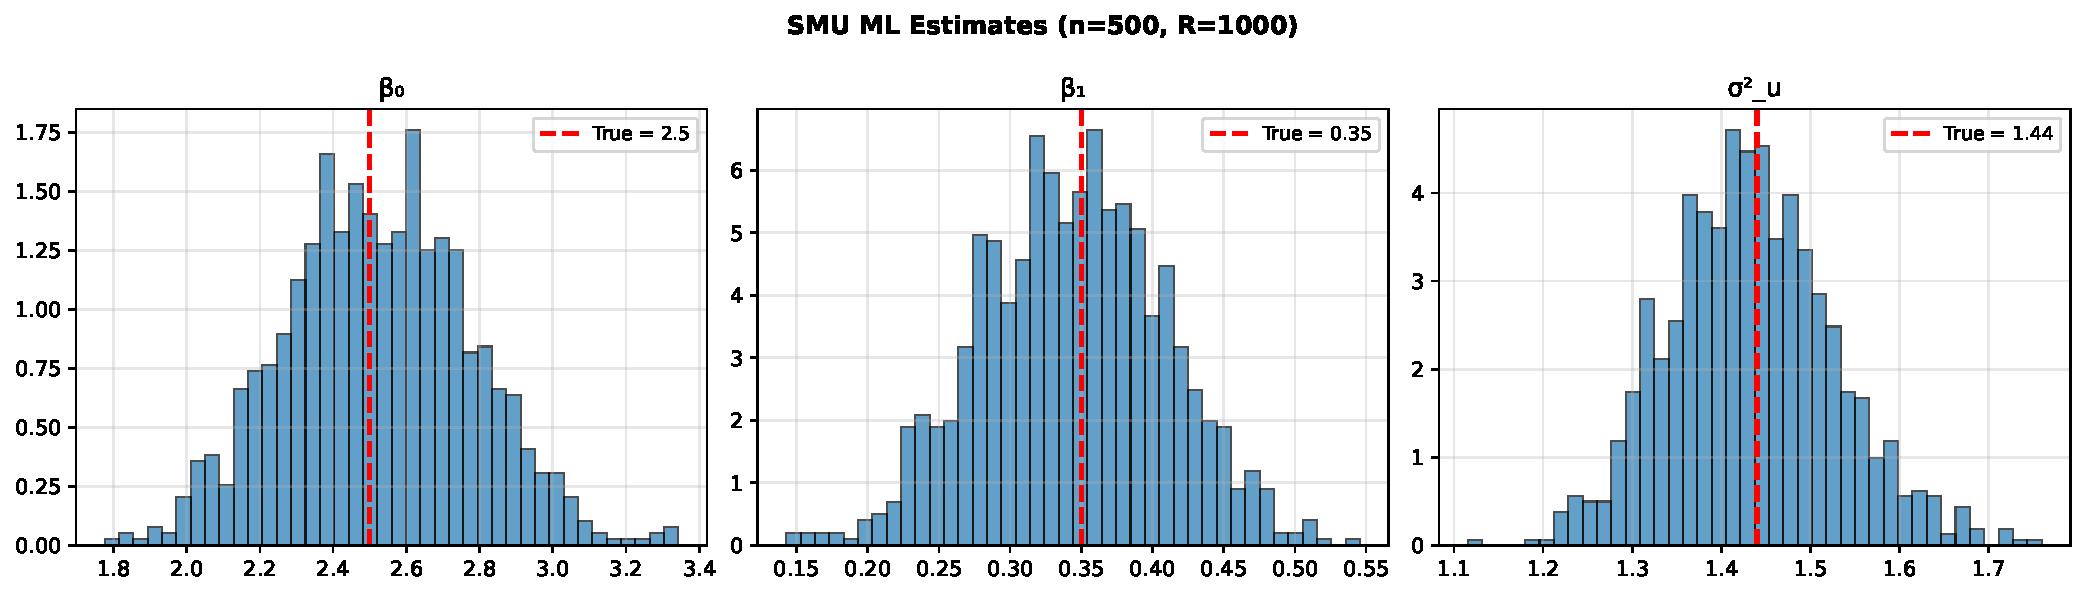
\includegraphics[width=\textwidth]{figures/mc_hist_smu_ml.pdf}
    \caption[Histograms of SMU ML estimates]{The figure shows histograms of $R = 1{,}000$ replications of SMU ML estimates. The true parameter values are marked by dashed red lines. We note that all three distributions are centred around the true value, showing approximate unbiasedness of the estimators.}
    \label{fig:mc_hist_smu_ml}
\end{figure}

\subsection{WB Equation}
\label{sec:mc:ml_wb}
Moving on to the WB equation, we apply Algorithm~\ref{alg:wb_ml}. Results are reported in Table~\ref{tab:mc_ml_results}, and histograms in Figure~\ref{fig:mc_hist_wb_ml}. The results are similar to those for the SMU equation: we have low bias, correspondence between standard errors, and good confidence interval coverage for all parameters, with the intercept $\gamma_0$ again showing higher bias and standard deviation. This is due to the same mechanism as before (see detailed explanation above for the SMU equation): the mean of the reduced form of $\vect{y}$ depends on $\gamma_0(1 - \gamma_3)^{-1}$, making the intercept partially confounded with the peer effect. Both the parameter $\gamma_2$ for the CoMO effect and $\gamma_3$ for the influence of peer WB are correctly estimated.

\begin{table}[htbp]
\centering
\caption[Monte Carlo results for WB ML estimator]{Monte Carlo results for WB ML estimator ($n = 500$, $R = 1{,}000$).}
\label{tab:mc_ml_results}
\begin{tabular}{lcccccc}
\toprule
Parameter & True & Mean Est. & Bias & Std(Est.) & Mean SE & Coverage \\
\midrule
$\gamma_0$ & 7.0 & 7.0306 & 0.0306 & 0.5050 & 0.5074 & 0.945 \\
$\gamma_1$ & $-0.5$ & $-0.4988$ & 0.0012 & 0.0538 & 0.0548 & 0.963 \\
$\gamma_2$ & $-0.8$ & $-0.7959$ & 0.0041 & 0.0938 & 0.0947 & 0.948 \\
$\gamma_3$ & 0.25 & 0.2442 & $-0.0058$ & 0.0623 & 0.0622 & 0.944 \\
$\sigma_\varepsilon^2$ & 1.00 & 0.9939 & $-0.0061$ & 0.0617 & 0.0632 & 0.956 \\
\bottomrule
\end{tabular}
\end{table}

\begin{figure}[htbp]
    \centering
    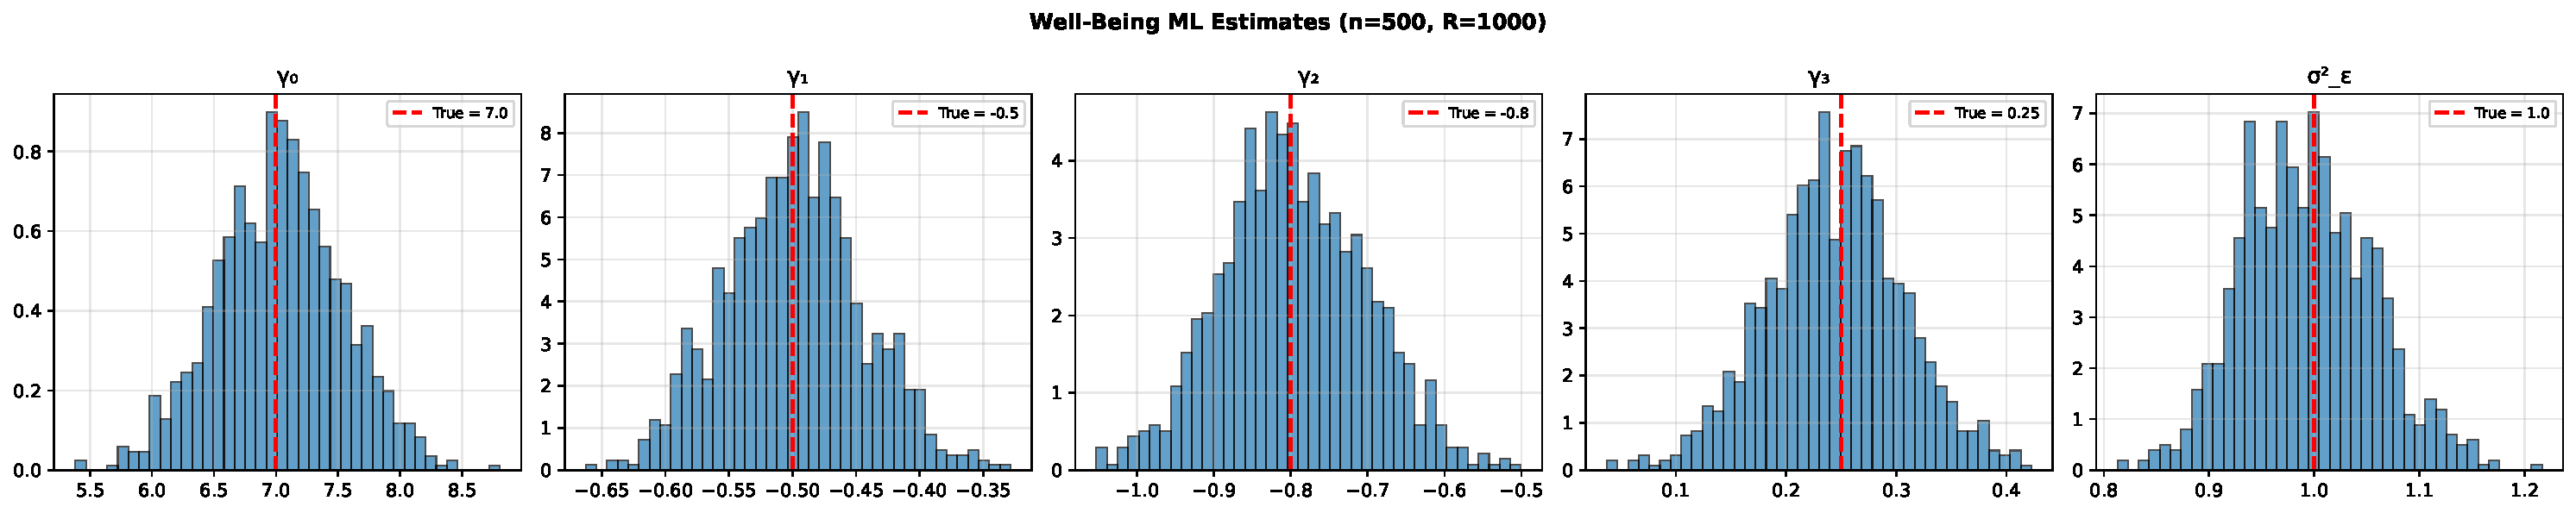
\includegraphics[width=\textwidth]{figures/mc_hist_wb_ml.pdf}
    \caption[Histograms of WB ML estimates]{Histograms of WB ML estimates across $R = 1{,}000$ replications. True parameter values shown as dashed red lines.}
    \label{fig:mc_hist_wb_ml}
\end{figure}

\subsection{Asymptotic Normality}
\label{sec:mc:normality}
We now validate the asymptotic normality of the ML estimators. Following the asymptotic theory of Section~\ref{sec:est:regularity} (see also Theorem~\ref{thm:mle_asymptotic}), we expect the standardised $z$-scores~\eqref{eq:mc_zscore_def} to be approximately $\N(0, 1)$-distributed.

For the WB equation, we plot histograms together with $\N(0, 1)$ overlays in Figure~\ref{fig:mc_zscore_hist}, and provide quantile-quantile plots in Figure~\ref{fig:mc_qq_ml}. Both show a close fit to the normal approximation for all estimated parameters. The empirical distributions follow the $\N(0, 1)$ reference closely, and the points in the Q-Q plots lie tightly along the diagonal with no evidence of heavy tails. These results confirm that the asymptotic approximation is adequate when $n = 500$.

\begin{figure}[htbp]
    \centering
    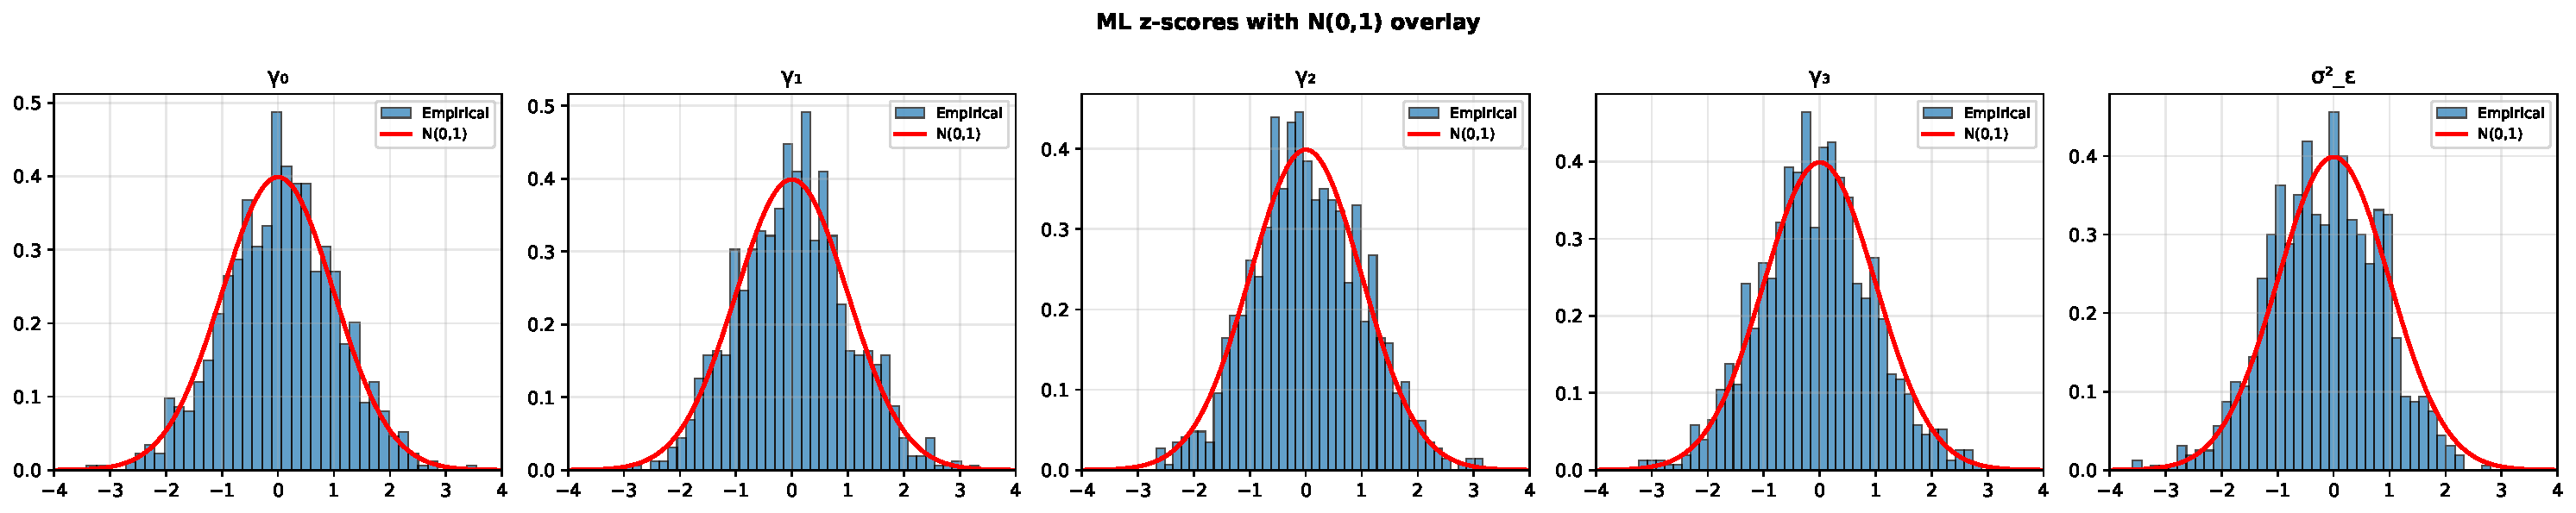
\includegraphics[width=\textwidth]{figures/mc_zscore_hist.pdf}
    \caption[Histograms of WB ML $z$-scores with $\N(0,1)$ overlays]{Histograms of ML $z$-scores with $\N(0,1)$ overlays (red curves) for each WB parameter.}
    \label{fig:mc_zscore_hist}
\end{figure}

\begin{figure}[htbp]
    \centering
    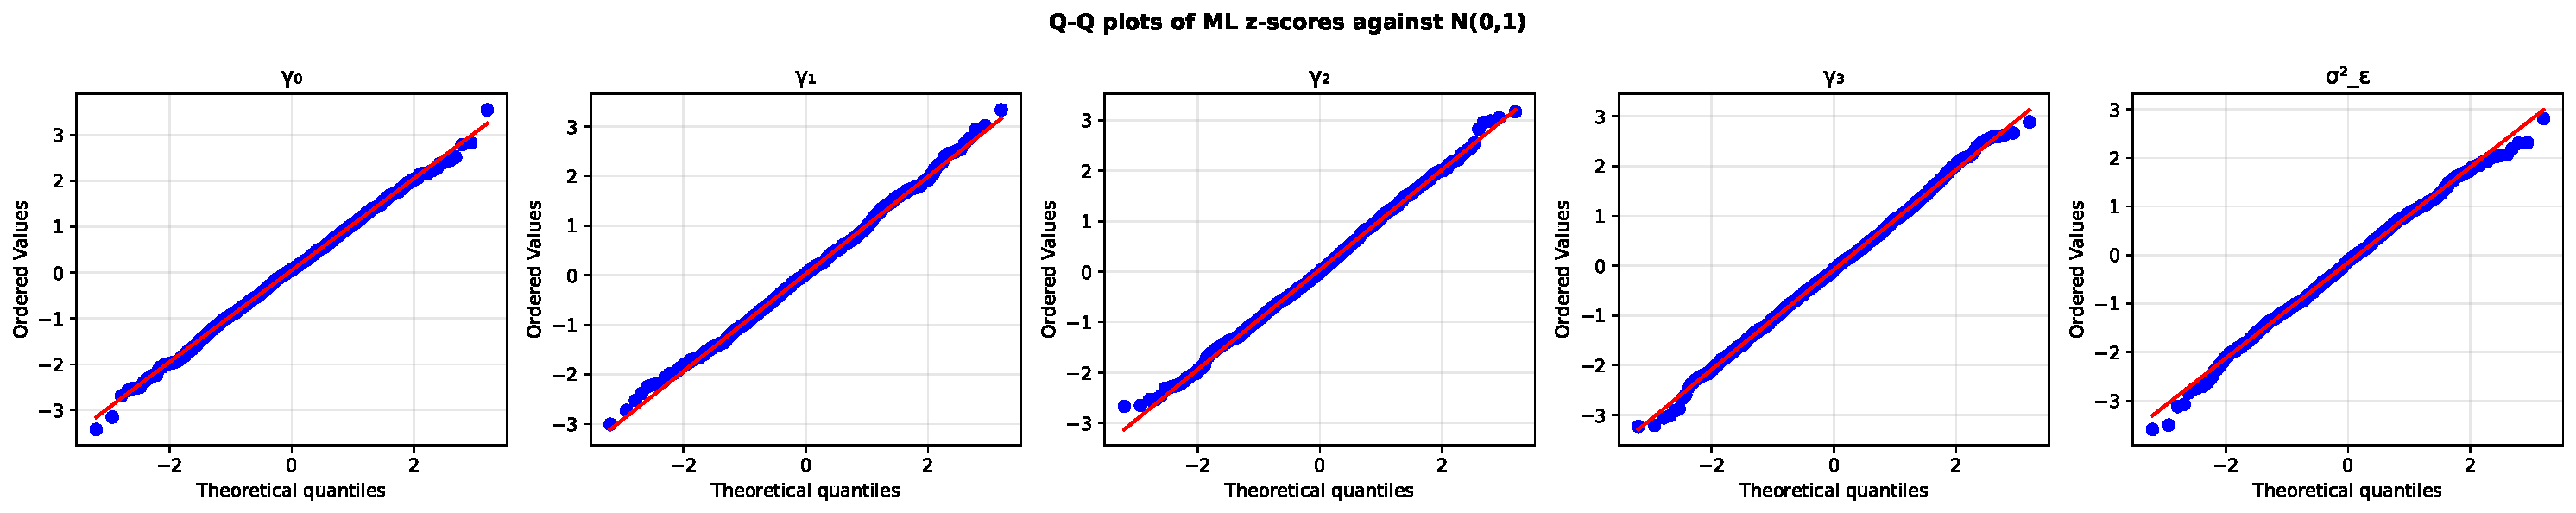
\includegraphics[width=\textwidth]{figures/mc_qq_ml.pdf}
    \caption[Q-Q plots of WB ML $z$-scores against $\N(0,1)$ quantiles]{Q-Q plots of empirical ML $z$-scores against the theoretical $\N(0,1)$ quantiles.}
    \label{fig:mc_qq_ml}
\end{figure}

We also provide an overview of summary statistics for the ML $z$-scores in Table~\ref{tab:mc_zscores_wb}. Here, all means are within $0.16$ of zero, and standard deviations within $0.02$ of $1$. This shows close correspondence with the theoretical mean of $0$ and standard deviation of $1$, respectively. The slightly larger discrepancy in the $\sigma_\varepsilon^2$ $z$-score mean (and similarly the $\sigma_u^2$ mean in Table~\ref{tab:mc_zscores_smu}) is consistent with general finite-sample downward bias of variance estimators for MLE \parencite[p.~331]{Casella2002}. The skewness and kurtosis are also negligible.

The ML $z$-scores for the SMU equation show similar results. For brevity, we omit the overlay and Q-Q plots, instead only reporting the summary statistics in Table~\ref{tab:mc_zscores_smu}. These also show a good correspondence with the expected theoretical values.

\begin{table}[htbp]
\centering
\caption[Summary statistics of WB ML $z$-scores]{Summary statistics of WB ML $z$-scores ($n = 500$, $R = 1{,}000$).}
\label{tab:mc_zscores_wb}
\begin{tabular}{lcccc}
\toprule
Parameter & Mean($z$) & Std($z$) & Skewness & Kurtosis \\
\midrule
$\gamma_0$ & 0.050 & 0.999 & $-0.070$ & 0.008 \\
$\gamma_1$ & 0.028 & 0.980 & 0.113 & $-0.098$ \\
$\gamma_2$ & 0.041 & 0.988 & 0.103 & $-0.139$ \\
$\gamma_3$ & $-0.079$ & 1.001 & 0.014 & 0.070 \\
$\sigma_\varepsilon^2$ & $-0.158$ & 0.983 & $-0.132$ & $-0.072$ \\
\bottomrule
\end{tabular}
\end{table}

\begin{table}[htbp]
\centering
\caption[Summary statistics of SMU ML $z$-scores]{Summary statistics of SMU ML $z$-scores ($n = 500$, $R = 1{,}000$).}
\label{tab:mc_zscores_smu}
\begin{tabular}{lcccc}
\toprule
Parameter & Mean($z$) & Std($z$) & Skewness & Kurtosis \\
\midrule
$\beta_0$ & 0.068 & 1.027 & $-0.059$ & $-0.123$ \\
$\beta_1$ & $-0.074$ & 1.028 & 0.095 & $-0.108$ \\
$\sigma_u^2$ & $-0.138$ & 1.023 & $-0.156$ & 0.192 \\
\bottomrule
\end{tabular}
\end{table}

%% Section 6.3: 2SLS Estimator Validation
\section{2SLS Estimator Validation}
\label{sec:mc:2sls}
In this section, we perform the Monte Carlo simulations validating the 2SLS estimator for the WB equation. A caveat on instrument strength should be kept in mind while reading this section. At the base $p = 0.01$ network density level, instrument strength is only moderate, with about $76\%$ of replications exceeding the \textcite[p.~557]{Staiger1997} threshold of $F = 10$. For the full diagnostics, see Section~\ref{sec:mc:first_stage}.

\subsection{Validation of the WB Equation}
\label{sec:mc:2sls_wb}
We now perform a Monte Carlo simulation to validate the 2SLS estimator of Section~\ref{sec:est:wb_2sls} for the WB equation, similar to that used for the ML estimator. We use the same instrument set as in~\eqref{eq:instrument_set}, $\mat{Z} = [\vect{1}, \vect{s}, \vect{c}, \mat{G}\vect{c}, \mat{G}^2\vect{s}, \mat{G}^2\vect{c}]$. We report the results in Table~\ref{tab:mc_2sls_results}, and display histograms of the estimates in Figure~\ref{fig:mc_hist_2sls}. Our results support the estimation strategy. Low bias, correspondence between empirical and HC1 standard errors, and coverage close to $95\%$ all indicate that the estimator is approximately unbiased and well-calibrated. We note that the coverage being consistently slightly above $95\%$ is in line with conservative standard errors when instrument strength is moderate (see Section~\ref{sec:mc:first_stage}).

We do not have a direct estimate of $\sigma_\varepsilon^2$ from the 2SLS estimator. If needed, we could obtain this indirectly from the residual variance. As we want to verify the 2SLS method specifically in this section, our results do not include this parameter.

\begin{table}[htbp]
\centering
\caption[Monte Carlo results for WB 2SLS estimator]{Monte Carlo results for WB 2SLS estimator ($n = 500$, $R = 1{,}000$).}
\label{tab:mc_2sls_results}
\begin{tabular}{lcccccc}
\toprule
Parameter & True & Mean Est. & Bias & Std(Est.) & Mean SE & Coverage \\
\midrule
$\gamma_0$ & 7.0 & 6.9227 & $-0.0773$ & 2.2312 & 2.2503 & 0.968 \\
$\gamma_1$ & $-0.5$ & $-0.4921$ & 0.0079 & 0.0792 & 0.0828 & 0.964 \\
$\gamma_2$ & $-0.8$ & $-0.7844$ & 0.0156 & 0.1125 & 0.1167 & 0.965 \\
$\gamma_3$ & 0.25 & 0.2564 & 0.0064 & 0.3138 & 0.3141 & 0.968 \\
\bottomrule
\end{tabular}
\end{table}

\begin{figure}[htbp]
    \centering
    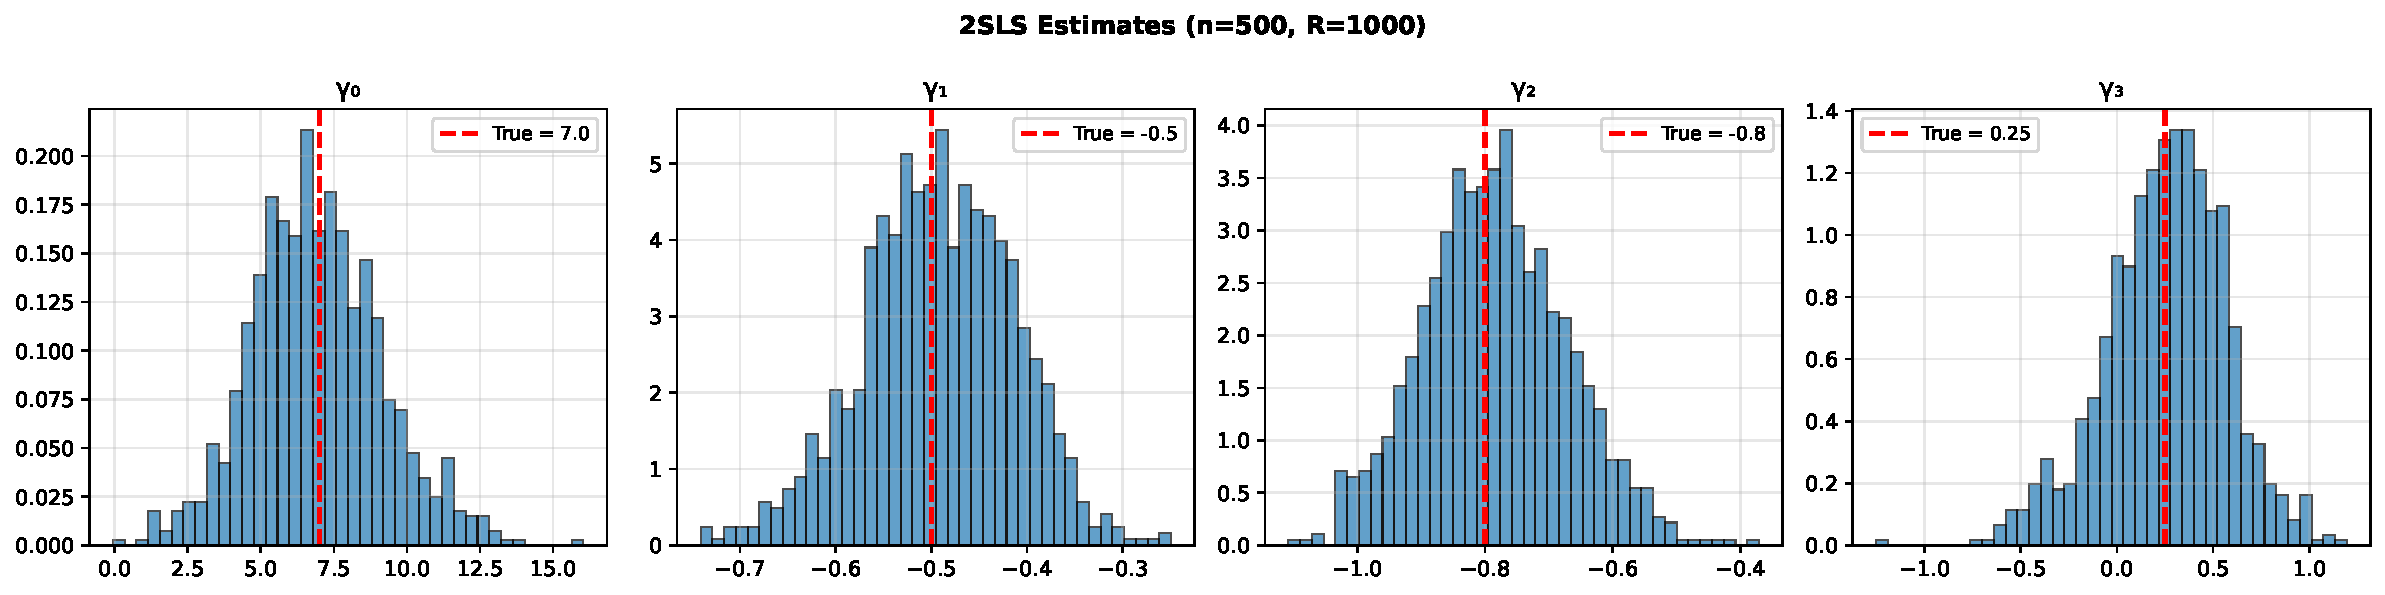
\includegraphics[width=\textwidth]{figures/mc_hist_2sls.pdf}
    \caption[Histograms of WB 2SLS estimates]{The figure shows histograms of 2SLS estimates from $R = 1{,}000$ Monte Carlo replications. We mark the true parameter values with dashed red lines.}
    \label{fig:mc_hist_2sls}
\end{figure}

\subsection{First-Stage Diagnostics}
\label{sec:mc:first_stage}
We now move on to tests and diagnostics of the 2SLS estimators (see Section~\ref{sec:est:diagnostics}), starting with the first-stage $F$-statistic.

This statistic tests the first stage of the 2SLS regression by checking whether the regression of $\mat{G}\vect{y}$ on $\mat{Z}$ has sufficient explanatory power. If it does not, we cannot expect 2SLS inference to be reliable. In our main Monte Carlo simulation for the 2SLS estimator, we thus also calculate the $F$-statistic for each of the $R = 1{,}000$ replications. A plot of the distribution of first-stage $F$-statistics is shown in Figure~\ref{fig:mc_fstat_hist}.

\begin{figure}[htbp]
    \centering
    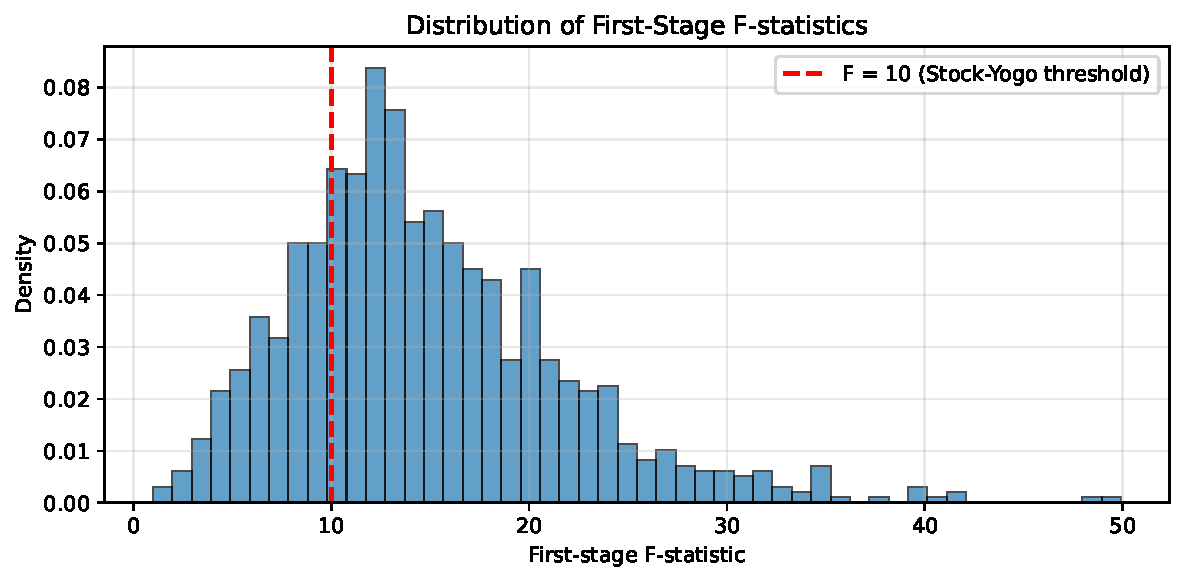
\includegraphics[width=0.8\textwidth]{figures/mc_fstat_hist.pdf}
    \caption[Distribution of first-stage $F$-statistics]{The figure plots the distribution of first-stage $F$-statistics for the $R = 1{,}000$ Monte Carlo replications. We mark the \textcite{Staiger1997} threshold of $F = 10$ with a dashed red line. Around $76\%$ of replications are above this threshold.}
    \label{fig:mc_fstat_hist}
\end{figure}

When interpreting these values, we follow the rule of thumb of \textcite{Staiger1997} and consider instruments that have $F < 10$ to be weak (for more details, see also the formal critical values of \textcite[Table~1]{StockYogo2005}). We report summary statistics including the fraction of replications with $F > 10$ in Table~\ref{tab:mc_fstat}.

\begin{table}[htbp]
\centering
\caption[First-stage $F$-statistic summary]{First-stage $F$-statistic summary ($n = 500$, $R = 1{,}000$).}
\label{tab:mc_fstat}
\begin{tabular}{lc}
\toprule
Statistic & Value \\
\midrule
Mean $F$ & 14.78 \\
Median $F$ & 13.55 \\
Fraction $F > 10$ & 0.759 \\
Fraction $F > 20$ & 0.202 \\
\bottomrule
\end{tabular}
\end{table}

Both the mean and median $F$-statistics of $14.78$ and $13.55$, respectively, are above the \textcite{Staiger1997} threshold of $10$. However, the fraction of $F$-statistics above $10$, at $75.9\%$, indicates that around $24\%$ of replications might have weak instruments. Based on this, we conclude that at $n = 500$ and $p = 0.01$, we have moderately strong instruments. In most replications, instruments are strong, and we obtain well-calibrated estimates in terms of bias and coverage. However, there are replications with weaker instruments, which might make 2SLS less efficient and thus the ML estimator preferable when the ML distributional requirements are met. This is also confirmed by the standard deviations, which are larger for the 2SLS estimates (Table~\ref{tab:mc_2sls_results}) than for the ML estimates (Table~\ref{tab:mc_ml_results}). The implication of these results is that researchers should take care to verify instrument strength before applying the 2SLS estimator.

\subsection{Overidentification and Hausman Tests}
\label{sec:mc:overid}
We now move on to the overidentification and Hausman tests (see Section~\ref{sec:est:diagnostics}). The results are calculated based on the same Monte Carlo simulation as before, with $n = 500$ and $R = 1{,}000$, and are reported in Table~\ref{tab:mc_diagnostics}.

As we have three excluded instruments and one endogenous regressor, our model is overidentified, and we can apply the Sargan--Hansen $J$-test. When all excluded instruments are valid, we have that $J \sim \chi^2_2$, and test rejection at the $5\%$ level should happen in approximately $5\%$ of replications. From Table~\ref{tab:mc_diagnostics}, we see that our Monte Carlo rejection rate is $4\%$, slightly below the expected value. The deviation is modest, about $1.5$ standard errors below the expected value when $R = 1{,}000$, and could thus reflect sampling variability. However, it might also indicate a mild effect from weak instruments in some of the replications, which would be in line with the observed first-stage $F$-statistics discussed above.

The Hausman test compares OLS and 2SLS estimates. Our DGP includes the endogenous $\mat{G}\vect{y}$ by construction, which means we expect a rejection rate higher than the nominal $5\%$ level, as the Hausman test should indicate the presence of endogeneity. However, the results reported in Table~\ref{tab:mc_diagnostics} show a Hausman rejection rate of $4.8\%$, close to the size expected under no endogeneity. With the other test results in mind, this result is not very surprising. The Hausman test does not have much power when the efficiency gap between OLS and 2SLS is high \parencite[p.~1258]{Hausman1978}. In our case, without very strong instruments, 2SLS is relatively imprecise, which makes the Hausman test statistic too noisy to separate the two estimators. However, as we will see in Section~\ref{sec:mc:ols_bias}, there is substantial bias in the OLS estimate $\hat\gamma_3$. Thus, the endogeneity present in our model still matters, even if the Hausman test does not have the power to detect it.

\begin{table}[htbp]
\centering
\caption[Diagnostic test rejection rates]{Diagnostic test rejection rates ($n = 500$, $R = 1{,}000$).}
\label{tab:mc_diagnostics}
\begin{tabular}{lcc}
\toprule
Test & Rejection Rate & Expected \\
\midrule
Sargan--Hansen $J$-test (H$_0$: instruments valid) & 0.040 & $\approx 0.05$ \\
Hausman test (H$_0$: no endogeneity) & 0.048 & $\gg 0.05$ \\
\bottomrule
\end{tabular}
\end{table}

\begin{remark}[Hausman Test Edge Case]
We include a reminder of the potential for the Hausman test statistic to be undefined in some cases due to the possibility of the difference $\widehat{\Var}(\hat{\gamma}_{\text{2SLS}}) - \widehat{\Var}(\hat{\gamma}_{\text{OLS}})$ in the denominator being negative in finite samples. Usually this should not occur, as 2SLS should have larger variance, but since the estimates are noisy, this might sometimes happen nonetheless. For our Monte Carlo run, this is not relevant, as it occurred in none of the $R = 1{,}000$ replications.
\end{remark}

\subsection{OLS Bias}
\label{sec:mc:ols_bias}
We end this section with a comparison to the OLS estimator. This estimator ignores the endogeneity of $\mat{G}\vect{y}$, which makes it biased compared to our ML and 2SLS estimators. The results for the (endogenous) $\gamma_3$ parameter are displayed in Table~\ref{tab:mc_ols_bias}. They show a much higher bias for OLS compared to the other two estimators. This is due to the simultaneity and network structure of our setup, which lead to a correlation between higher $\mat{G}\vect{y}$ and higher $\varepsilon_i$. OLS ends up with an inflated estimate of the peer effect, while our ML and 2SLS estimators correctly handle the endogenous regressor.

\begin{table}[htbp]
\centering
\caption[OLS, ML, and 2SLS bias comparison for $\gamma_3$]{OLS, ML, and 2SLS bias comparison for $\gamma_3$ ($n = 500$, $R = 1{,}000$).}
\label{tab:mc_ols_bias}
\begin{tabular}{lccc}
\toprule
Method & Mean $\hat\gamma_3$ & Bias & RMSE \\
\midrule
OLS & 0.4050 & 0.1550 & 0.1852 \\
ML & 0.2442 & $-0.0058$ & 0.0625 \\
2SLS & 0.2564 & 0.0064 & 0.3139 \\
\bottomrule
\end{tabular}
\end{table}

%% Section 6.4: Comparison of ML and 2SLS
\section{Comparison of ML and 2SLS}
\label{sec:mc:comparison}
We have validated both the ML and 2SLS estimators. Now we will compare their performance in finite samples for the WB equation. This will give us insight into when it is preferable to use one or the other. This section builds on the theoretical comparison of Section~\ref{sec:est:comparison}.

We begin with a comparison of the bias and efficiency of the estimators. As we are working under an assumption of normality, we expect the ML estimator to outperform the 2SLS estimator. This is exactly what we find. In Table~\ref{tab:mc_comparison}, we report the bias and RMSE comparison of the two methods, along with a measure of relative efficiency, defined as $\text{RMSE}_{\text{2SLS}} / \text{RMSE}_{\text{ML}}$. Under normality, the relative efficiency should be $\geq 1$ for all parameters, as the ML estimator is more efficient than 2SLS, with magnitude depending on instrument strength. Our results show a lower bias for the ML estimator across the board, and relative efficiencies ranging from around $1.2$ to $5.0$. The highest relative efficiencies are for $\gamma_0$ ($4.41$) and $\gamma_3$ ($5.02$). The latter corresponds well with the previous test result showing that the instruments are only moderately strong. For $\gamma_0$, the efficiency gap can be explained by the intercept identification issue discussed in Section~\ref{sec:mc:ml_wb}.

\begin{table}[htbp]
\centering
\caption[ML vs.\ 2SLS comparison for the WB equation]{ML vs.\ 2SLS comparison for the WB equation ($n = 500$, $R = 1{,}000$).}
\label{tab:mc_comparison}
\begin{tabular}{lccccc}
\toprule
 & \multicolumn{2}{c}{Bias} & \multicolumn{2}{c}{RMSE} & Relative \\
\cmidrule(lr){2-3} \cmidrule(lr){4-5}
Parameter & ML & 2SLS & ML & 2SLS & Efficiency \\
\midrule
$\gamma_0$ & 0.0306 & $-0.0773$ & 0.5059 & 2.2325 & 4.41 \\
$\gamma_1$ & 0.0012 & 0.0079 & 0.0539 & 0.0796 & 1.48 \\
$\gamma_2$ & 0.0041 & 0.0156 & 0.0939 & 0.1136 & 1.21 \\
$\gamma_3$ & $-0.0058$ & 0.0064 & 0.0625 & 0.3139 & 5.02 \\
\bottomrule
\end{tabular}
\end{table}

We further compare ML and 2SLS through scatter plots of the estimates in Figure~\ref{fig:mc_ml_vs_2sls_scatter}. Here, agreement corresponds to a clustering of points around the identity line, which would indicate that the estimators recover the same underlying parameters. We see a relatively good correspondence between the estimators for the $\gamma_1$ and $\gamma_2$ parameters, with a difference for the $\gamma_3$ parameter. This is due to the higher efficiency of the ML estimator for this parameter, making the ML points cluster more tightly around the true value.

\begin{figure}[htbp]
    \centering
    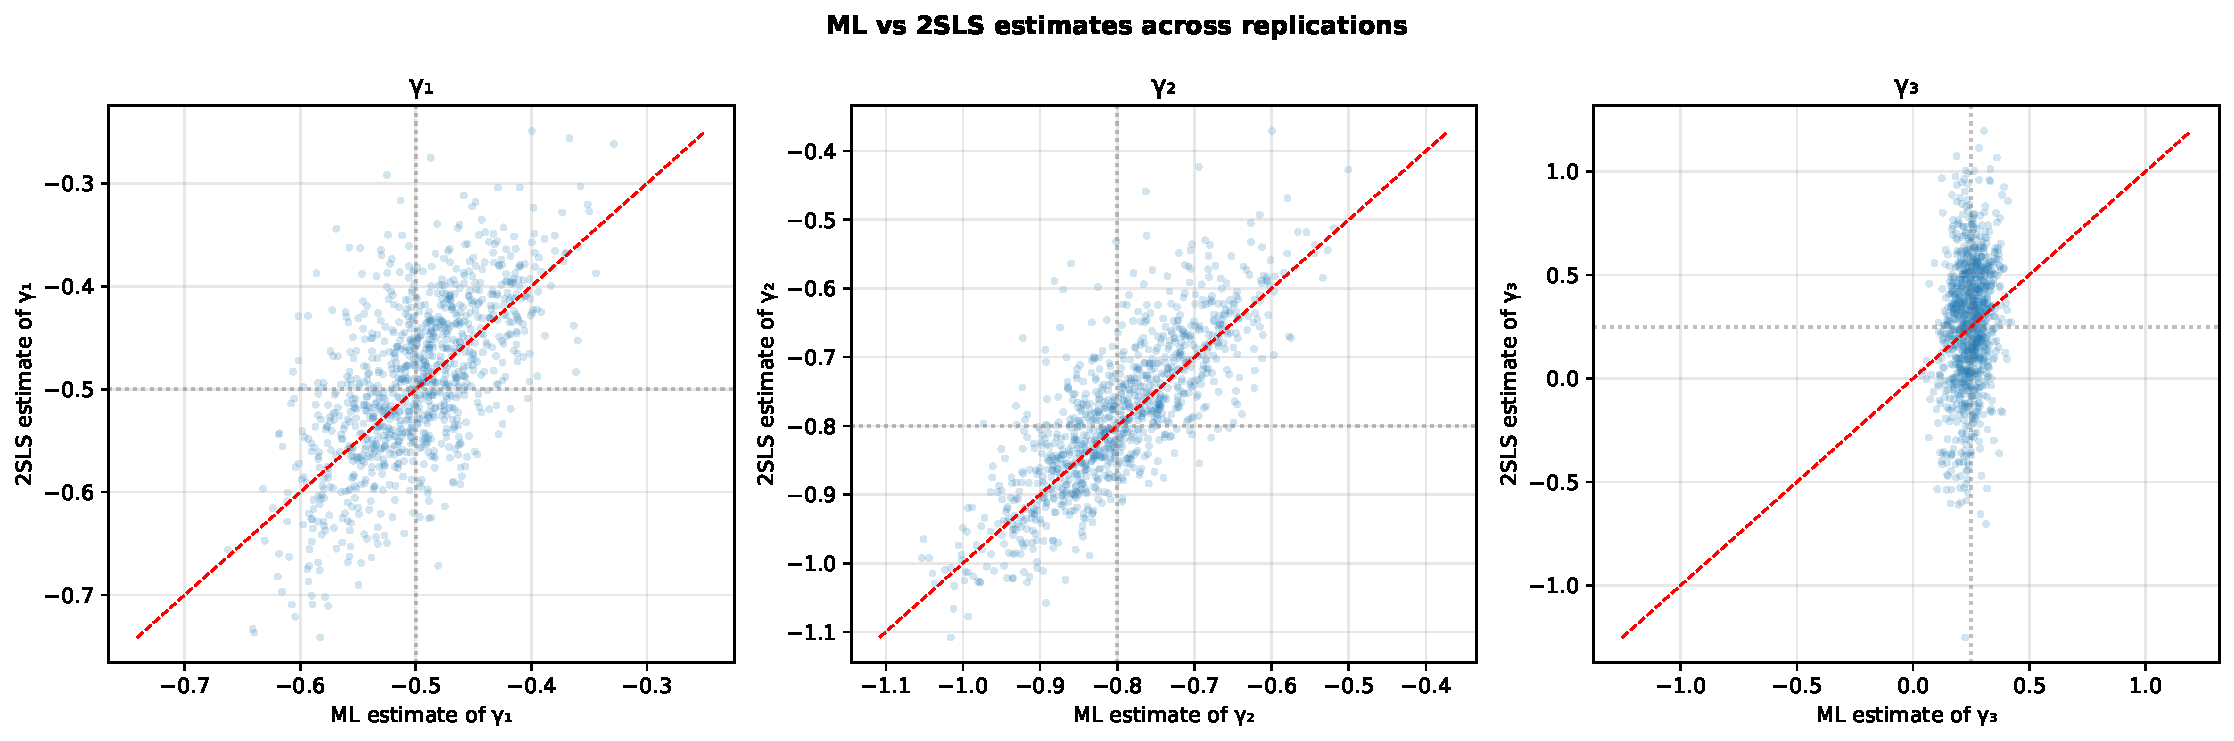
\includegraphics[width=\textwidth]{figures/mc_ml_vs_2sls_scatter.pdf}
    \caption[Scatter plots of ML vs.\ 2SLS estimates]{Scatter plots of ML vs.\ 2SLS estimates for $\gamma_1$, $\gamma_2$, and $\gamma_3$ across the Monte Carlo replications. The dashed red line is the identity line. We note a higher variance for the 2SLS estimates, especially for $\gamma_3$.}
    \label{fig:mc_ml_vs_2sls_scatter}
\end{figure}

%% Section 6.5: Wald Test Calibration
\section{Wald Test Calibration}
\label{sec:mc:wald}
In Section~\ref{sec:est:testing}, we developed a Wald test for the CoMO coefficient $\gamma_2$, and a joint Wald test for the network-term coefficients $\gamma_2$ and $\gamma_3$. This section validates these. The two null hypotheses are
\begin{align}
    H_0^{(a)}&: \gamma_2 = 0 \quad \text{(no CoMO effect, single Wald test)}, \\
    H_0^{(b)}&: \gamma_2 = \gamma_3 = 0 \quad \text{(no network effects, joint Wald test)}.
\end{align}

We evaluate the empirical sizes of the tests: the number of times they reject under the null hypotheses, for both the ML and the 2SLS covariance estimators. The Hessian-based standard errors of~\eqref{eq:se_formula} are used for the ML approach, where the analytical observed information matrix of Section~\ref{sec:est:wb_hessian} is inverted, and the $(\gamma_2, \gamma_3)$ block is extracted. The corresponding block of the HC1-robust sandwich matrix from~\eqref{eq:robust_se} is used for 2SLS\@. Using these, we can compute the test for $\gamma_2$ as $t = \hat\gamma_2 / \widehat{\text{SE}}(\hat\gamma_2)$ and for $\gamma_2$ and $\gamma_3$ as $W = \hat{\gammavec}_R^\top [\mat{R}\,\widehat{\Var}(\hat{\thetavec}_y)\,\mat{R}^\top]^{-1} \hat{\gammavec}_R$ (see Section~\ref{sec:est:testing}). These statistics are asymptotically standard-normal and $\chi^2_2$ distributed, respectively.

The Monte Carlo simulations are run with $n = 500$, $p = 0.01$, $R = 1{,}000$, and network generation as in Section~\ref{sec:mc:procedure}. The null DGP uses the same parameters as in Table~\ref{tab:mc_true_params} except that we set $\gamma_2 = \gamma_3 = 0$. We use this same DGP for both tests, as it satisfies both null hypotheses. We do not verify the size of the single-hypothesis test when $\gamma_3 \neq 0$ here. We compare the sizes to the nominal level of $\alpha = 0.05$. The rejection rates are reported in Table~\ref{tab:mc_wald}. We also show the empirical cumulative distribution functions (CDFs) of the joint Wald $p$-values in Figure~\ref{fig:mc_wald_pvalues}. Under correct calibration, these should lie on 45-degree lines in the plots.

\begin{table}[htbp]
\centering
\caption[Wald test size]{Wald test size ($n = 500$, $R = 1{,}000$, $\alpha = 0.05$). Size is the rejection rate under the null DGP ($\gamma_2 = \gamma_3 = 0$).}
\label{tab:mc_wald}
\begin{tabular}{llc}
\toprule
Estimator & Test (null hypothesis) & Size \\
\midrule
ML   & Single $(H_0: \gamma_2 = 0)$              & 0.050 \\
ML   & Joint  $(H_0: \gamma_2 = \gamma_3 = 0)$   & 0.045 \\
2SLS & Single $(H_0: \gamma_2 = 0)$              & 0.041 \\
2SLS & Joint  $(H_0: \gamma_2 = \gamma_3 = 0)$   & 0.038 \\
\bottomrule
\end{tabular}
\end{table}

\begin{figure}[htbp]
    \centering
    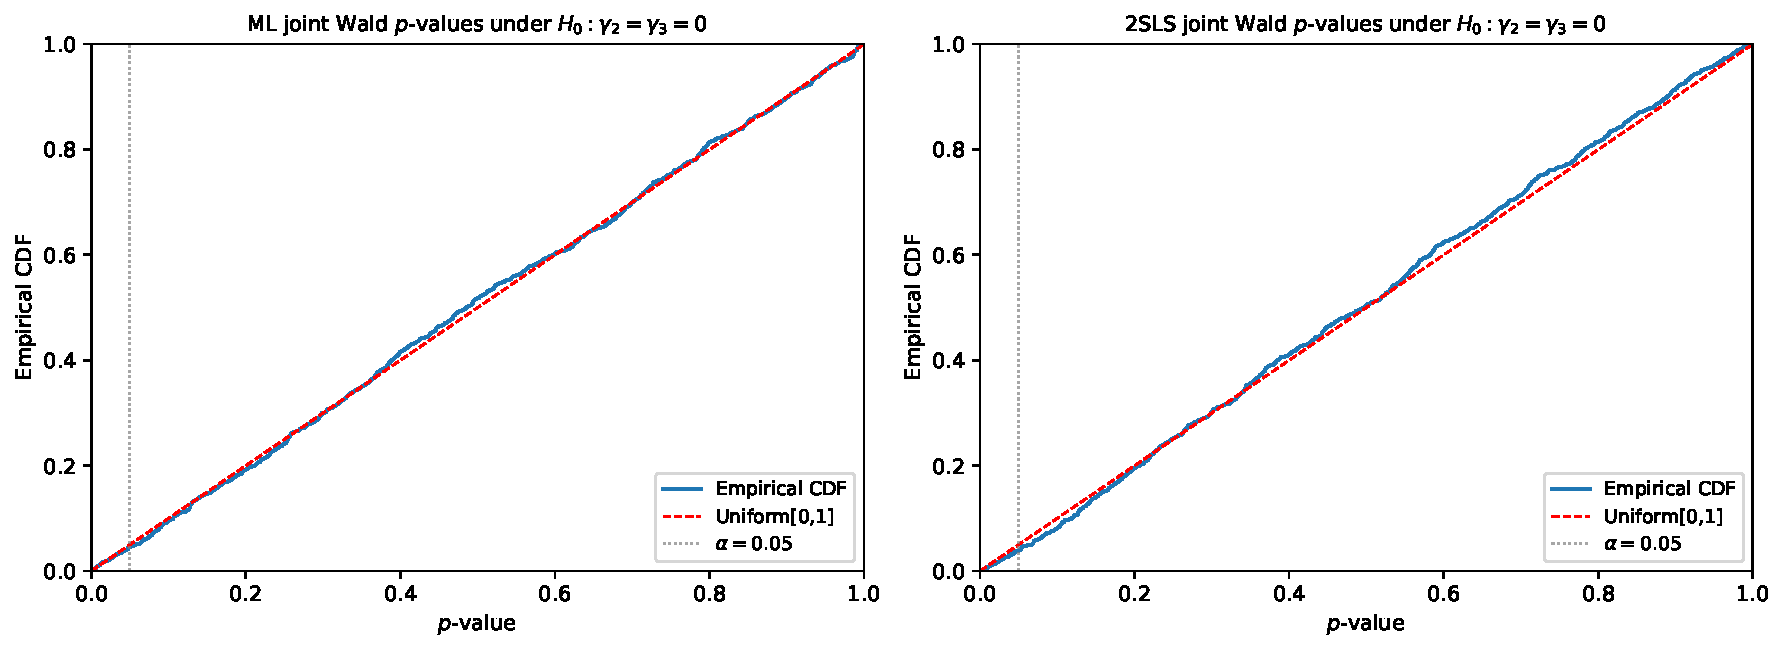
\includegraphics[width=\textwidth]{figures/mc_wald_pvalues.pdf}
    \caption[Empirical CDFs of joint Wald $p$-values under the null]{The plots show empirical CDFs of joint Wald $p$-values under the null DGP, with covariance estimators for ML in the left panel, and 2SLS in the right panel. We mark the theoretical $\text{Uniform}[0, 1]$ CDF with a red dashed line. The dotted vertical line shows the nominal level $\alpha = 0.05$ used for reporting the values in Table~\ref{tab:mc_wald}.}
    \label{fig:mc_wald_pvalues}
\end{figure}

The results show a good calibration under the null across the four tests. For $R = 1{,}000$ replications, the Monte Carlo standard error of a rejection rate near $0.05$ is $\sqrt{0.05 \times 0.95 / 1{,}000} \approx 0.007$. This gives the two-standard-error band of $0.036$ to $0.064$ around the nominal level. All sizes are within this band, with the ML rejection rates of $0.050$ and $0.045$ being very close to nominal, and the 2SLS rejection rates of $0.041$ and $0.038$ being slightly below it. The mild under-rejection of 2SLS might be explained by the HC1 standard errors being conservative (see Section~\ref{sec:mc:2sls}). The CDF plots of Figure~\ref{fig:mc_wald_pvalues} confirm the good calibration, with empirical CDFs close to the expected 45-degree lines. Together with the $z$-score analysis of Section~\ref{sec:mc:normality}, these results provide evidence that the asymptotic approximations of Section~\ref{sec:est:testing} hold when $n = 500$.

We do not include an empirical power study here, as at the current DGP the coefficients are large enough that single-point power is uninformative. A comparable power analysis for the nested Wald test in the simultaneous CoMO model is reported in Section~\ref{sec:simul:wald_test}.

%% Section 6.6: Effect of Network Density
\section{Effect of Network Density}
\label{sec:mc:density}
Differences in network density can affect the performance of estimators. Because of this, we include a section testing estimator robustness under varying network densities.

When network density changes, this also changes the number of connections per individual in the network. As $\mat{G}$ is row-normalised, this leads to neighbour averages being computed over a different number of neighbours, which in turn affects $\mat{G}\vect{y}$. With higher density, this term becomes more homogeneous, which can make instruments weaker and hence also degrade the performance of 2SLS estimators.

To investigate the effect of network density, we perform Monte Carlo simulations with varying levels of the connection probability $p$:
\begin{equation}
    p \in \{0.01, 0.02, 0.03, 0.05, 0.10\}
\end{equation}

We use $n = 500$ individuals, and thus get the expected degrees of approximately $5$, $10$, $15$, $25$, and $50$ for these networks. This creates examples ranging from a moderately sparse network to a relatively homogeneous one, allowing us to properly test our estimators. To reduce the computational burden, we lower the number of replications to $R = 500$ (from $R = 1{,}000$ previously). Otherwise, we keep the exact same DGP parameters as before (see Table~\ref{tab:mc_true_params}). We focus on the $\gamma_2$ and $\gamma_3$ parameters, as their identification depends most directly on the network structure. When changing $\mat{G}$ and the instruments derived from it, these are thus the most informative parameters to track. The remaining parameters are less sensitive to the network structure.

The main results are covered in Tables~\ref{tab:mc_density_g2} and~\ref{tab:mc_density_g3}, with corresponding plots in Figure~\ref{fig:mc_density_sensitivity}. We also report the mean first-stage $F$-statistic at each density, along with a verification that the Bramoull\'e identification condition (linear independence of $\mat{I}$, $\mat{G}$, and $\mat{G}^2$) holds, in Table~\ref{tab:mc_identification}.

\begin{table}[htbp]
\centering
\caption[Effect of network density on $\gamma_2$ estimation]{Effect of network density on $\gamma_2$ estimation ($n = 500$, $R = 500$).}
\label{tab:mc_density_g2}
\begin{tabular}{lccccccc}
\toprule
 & & \multicolumn{3}{c}{ML} & \multicolumn{3}{c}{2SLS} \\
\cmidrule(lr){3-5} \cmidrule(lr){6-8}
$p$ & Exp.\ Degree & Bias & RMSE & Coverage & Bias & RMSE & Coverage \\
\midrule
0.01 & 5 & $-0.0061$ & 0.0959 & 0.946 & 0.0060 & 0.1172 & 0.946 \\
0.02 & 10 & 0.0030 & 0.1053 & 0.948 & 0.0159 & 0.1228 & 0.946 \\
0.03 & 15 & 0.0052 & 0.1143 & 0.952 & 0.0194 & 0.1286 & 0.950 \\
0.05 & 25 & 0.0054 & 0.1210 & 0.944 & 0.0243 & 0.1345 & 0.962 \\
0.10 & 50 & 0.0052 & 0.1250 & 0.940 & 0.0166 & 0.1350 & 0.950 \\
\bottomrule
\end{tabular}
\end{table}

\begin{table}[htbp]
\centering
\caption[Effect of network density on $\gamma_3$ estimation]{Effect of network density on $\gamma_3$ estimation ($n = 500$, $R = 500$).}
\label{tab:mc_density_g3}
\begin{tabular}{lccccccc}
\toprule
 & & \multicolumn{3}{c}{ML} & \multicolumn{3}{c}{2SLS} \\
\cmidrule(lr){3-5} \cmidrule(lr){6-8}
$p$ & Exp.\ Degree & Bias & RMSE & Coverage & Bias & RMSE & Coverage \\
\midrule
0.01 & 5 & $-0.0087$ & 0.0633 & 0.942 & 0.0151 & 0.3047 & 0.962 \\
0.02 & 10 & $-0.0138$ & 0.0900 & 0.956 & 0.0134 & 0.6636 & 0.956 \\
0.03 & 15 & $-0.0229$ & 0.1101 & 0.972 & 0.0538 & 0.9472 & 0.964 \\
0.05 & 25 & $-0.0328$ & 0.1473 & 0.962 & 0.2460 & 1.6079 & 0.968 \\
0.10 & 50 & $-0.0637$ & 0.2157 & 0.938 & 0.4487 & 2.7588 & 0.980 \\
\bottomrule
\end{tabular}
\end{table}


\begin{table}[htbp]
\centering
\caption[Identification condition check and mean first-stage $F$-statistics]{Identification condition check and mean first-stage $F$-statistics ($n = 500$, $R = 500$).}
\label{tab:mc_identification}
\begin{tabular}{lcc}
\toprule
$p$ & Fraction with rank$[\mat{I}, \mat{G}, \mat{G}^2] = 3$ & Mean first-stage $F$ \\
\midrule
0.01 & 1.00 & 15.36 \\
0.02 & 1.00 & 8.95 \\
0.03 & 1.00 & 6.70 \\
0.05 & 1.00 & 4.91 \\
0.10 & 1.00 & 3.48 \\
\bottomrule
\end{tabular}
\end{table}

We first note the results of Table~\ref{tab:mc_identification}: the identification condition holds for all networks, and there is a decline in the mean first-stage $F$-statistic as network density grows. This is because the network becomes more homogeneous, leading instrument strength to decrease as less variation can be provided by the network structure. We now discuss the effect this has on our parameter estimates.

For the $\gamma_2$ parameter for the CoMO effect, both estimators perform well under the varying network densities. We find this in both Table~\ref{tab:mc_density_g2} and the plots of Figure~\ref{fig:mc_density_sensitivity} (top row). While we do observe a slightly degraded performance for denser networks in terms of an increase in RMSE (and, arguably, for the bias of the 2SLS estimator), the increase is not drastic. Both estimators have low bias and relatively good coverage at all simulated network densities.

The $\gamma_3$ parameter corresponding to the endogenous term tells a different story. As reported in Table~\ref{tab:mc_density_g3} and seen in Figure~\ref{fig:mc_density_sensitivity} (bottom row), the performance of the two estimators diverges as the density of the network grows. For the ML estimator, we observe a slight to moderate increase in both bias and RMSE as the density grows, with coverage staying near the nominal level. Thus, the performance degrades slightly with network density, but we still recover the parameter with low bias and standard deviation. The slight increase in ML bias for the $\gamma_3$ parameter might be caused by denser networks making $\mat{G}$ closer to a rank-one matrix, implying less curvature from the Jacobian term. This makes identifying $\gamma_3$ harder, as it becomes more confounded with the intercept. The 2SLS estimator, on the other hand, exhibits a sharp increase in both bias and RMSE as the network density increases. The coverage does stay close to nominal, but this might be due to increasingly wide confidence intervals, not actual performance, as the RMSE for $\hat\gamma_3$ increases by around an order of magnitude across the density range. The degradation of the 2SLS estimator is much more pronounced than for the ML estimator. This corresponds well with our previous reasoning: as the network density grows, the network becomes more homogeneous, weakening instrument strength. Homogeneous, well-connected networks do not provide the same network-based variation as sparse networks do, leading to a degradation of the 2SLS estimates. This is consistent with the observed decline in the $F$-statistics (Table~\ref{tab:mc_identification}).

\begin{figure}[htbp]
    \centering
    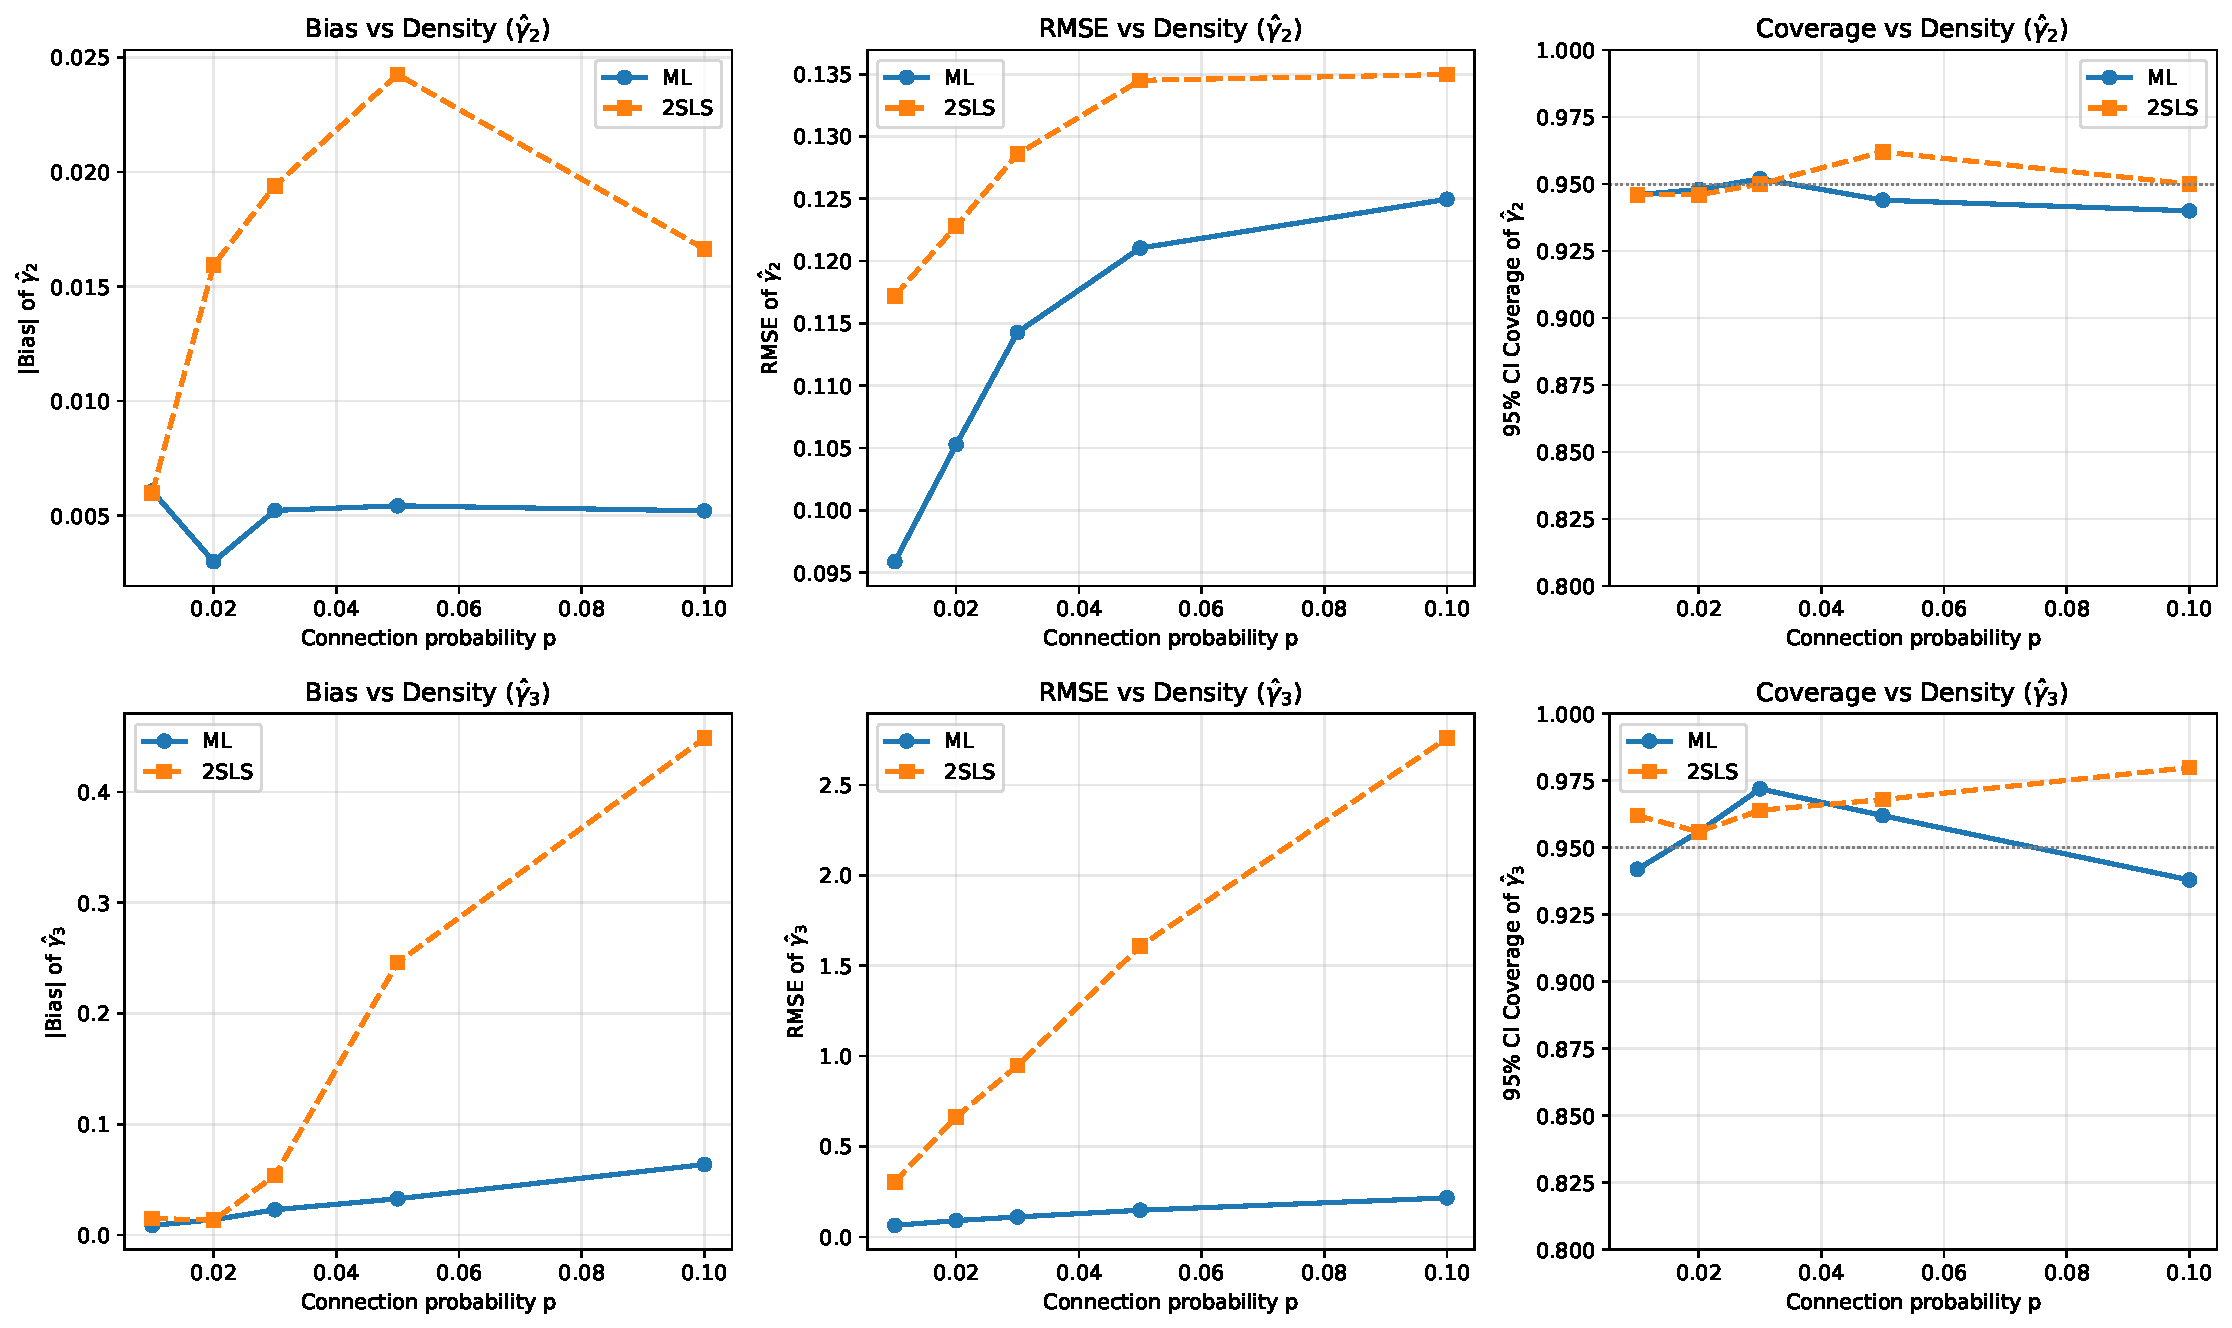
\includegraphics[width=\textwidth]{figures/mc_density_sensitivity.pdf}
    \caption[Effect of network density on bias, RMSE, and CI coverage]{We plot the effect of network density on absolute bias, RMSE, and $95\%$ CI coverage for $\hat\gamma_2$ (top row) and $\hat\gamma_3$ (bottom row). There is a stark difference between the ML and 2SLS performance for the endogenous $\gamma_3$ parameter.}
    \label{fig:mc_density_sensitivity}
\end{figure}

The results of our Monte Carlo simulations on network density show a divergence between the ML and 2SLS estimators. When networks are sparse, both estimators can be successfully applied. However, as density grows, the mean $F$-statistic quickly falls below the \textcite{Staiger1997} threshold of $10$. The 2SLS estimator degrades as weak-instrument issues arise. This leads to the following conclusion: for sparse networks, both the ML and 2SLS estimators can be applied, while in settings with denser networks, ML is preferred.

%% Section 6.7: Convergence as Sample Size Increases
\section{Convergence as Sample Size Increases}
\label{sec:mc:convergence}
Lastly, we perform simulations investigating the convergence as the sample size increases. We do this by increasing the size of the network while holding the expected degree constant. Keeping the degree constant allows us to isolate the effect of increased sample size, giving a complementary study to the density study of Section~\ref{sec:mc:density}. If the estimators work as expected, we should observe improved performance as $n$ grows.

To perform the simulations, we fix the expected degree at $10$ and simulate for the following sample sizes:
\begin{equation}
    n \in \{500, 750, 1{,}000, 1{,}500, 2{,}000\}
\end{equation}

To keep the expected degree fixed, we need to scale the connection probability $p$ as the network size increases. Setting $p = 10/(n-1)$, we get approximately $10$ as the expected number of connections per individual, along with $p \approx 0.020, 0.013, 0.010, 0.007, 0.005$ for the five sample sizes. Otherwise, we use the same DGP parameters as before (see Table~\ref{tab:mc_true_params}), and use $R = 500$ Monte Carlo replications.

As with the density study, we report results for the $\gamma_2$ and $\gamma_3$ parameters, since these are the most network-dependent and hence the most informative to investigate (see discussion in Section~\ref{sec:mc:density}). We report the results for $\gamma_2$ in Table~\ref{tab:mc_convergence_g2} and for $\gamma_3$ in Table~\ref{tab:mc_convergence_g3}, along with log-log plots of convergence for both in Figure~\ref{fig:mc_convergence}.

\begin{table}[htbp]
\centering
\caption[Convergence of ML and 2SLS estimators for $\gamma_2$]{Convergence of ML and 2SLS estimators for $\gamma_2$ (True = $-0.8$, $R = 500$).}
\label{tab:mc_convergence_g2}
\begin{tabular}{lccccccc}
\toprule
 & & \multicolumn{3}{c}{ML} & \multicolumn{3}{c}{2SLS} \\
\cmidrule(lr){3-5} \cmidrule(lr){6-8}
$n$ & $p$ & Bias & RMSE & Coverage & Bias & RMSE & Coverage \\
\midrule
500 & 0.0200 & $-0.0059$ & 0.1034 & 0.960 & 0.0084 & 0.1187 & 0.968 \\
750 & 0.0134 & 0.0008 & 0.0927 & 0.926 & 0.0124 & 0.1038 & 0.952 \\
1{,}000 & 0.0100 & 0.0007 & 0.0781 & 0.946 & 0.0072 & 0.0887 & 0.940 \\
1{,}500 & 0.0067 & 0.0012 & 0.0625 & 0.946 & 0.0072 & 0.0703 & 0.952 \\
2{,}000 & 0.0050 & 0.0032 & 0.0556 & 0.946 & 0.0055 & 0.0627 & 0.942 \\
\bottomrule
\end{tabular}
\end{table}

\begin{table}[htbp]
\centering
\caption[Convergence of ML and 2SLS estimators for $\gamma_3$]{Convergence of ML and 2SLS estimators for $\gamma_3$ (True = $0.25$, $R = 500$).}
\label{tab:mc_convergence_g3}
\begin{tabular}{lccccccc}
\toprule
 & & \multicolumn{3}{c}{ML} & \multicolumn{3}{c}{2SLS} \\
\cmidrule(lr){3-5} \cmidrule(lr){6-8}
$n$ & $p$ & Bias & RMSE & Coverage & Bias & RMSE & Coverage \\
\midrule
500 & 0.0200 & $-0.0096$ & 0.0920 & 0.956 & 0.0350 & 0.6827 & 0.962 \\
750 & 0.0134 & $-0.0167$ & 0.0783 & 0.946 & 0.0357 & 0.4970 & 0.954 \\
1{,}000 & 0.0100 & $-0.0106$ & 0.0668 & 0.946 & $-0.0084$ & 0.4552 & 0.966 \\
1{,}500 & 0.0067 & $-0.0027$ & 0.0556 & 0.942 & 0.0120 & 0.3549 & 0.954 \\
2{,}000 & 0.0050 & $-0.0003$ & 0.0458 & 0.950 & $-0.0051$ & 0.3082 & 0.968 \\
\bottomrule
\end{tabular}
\end{table}

\begin{figure}[htbp]
    \centering
    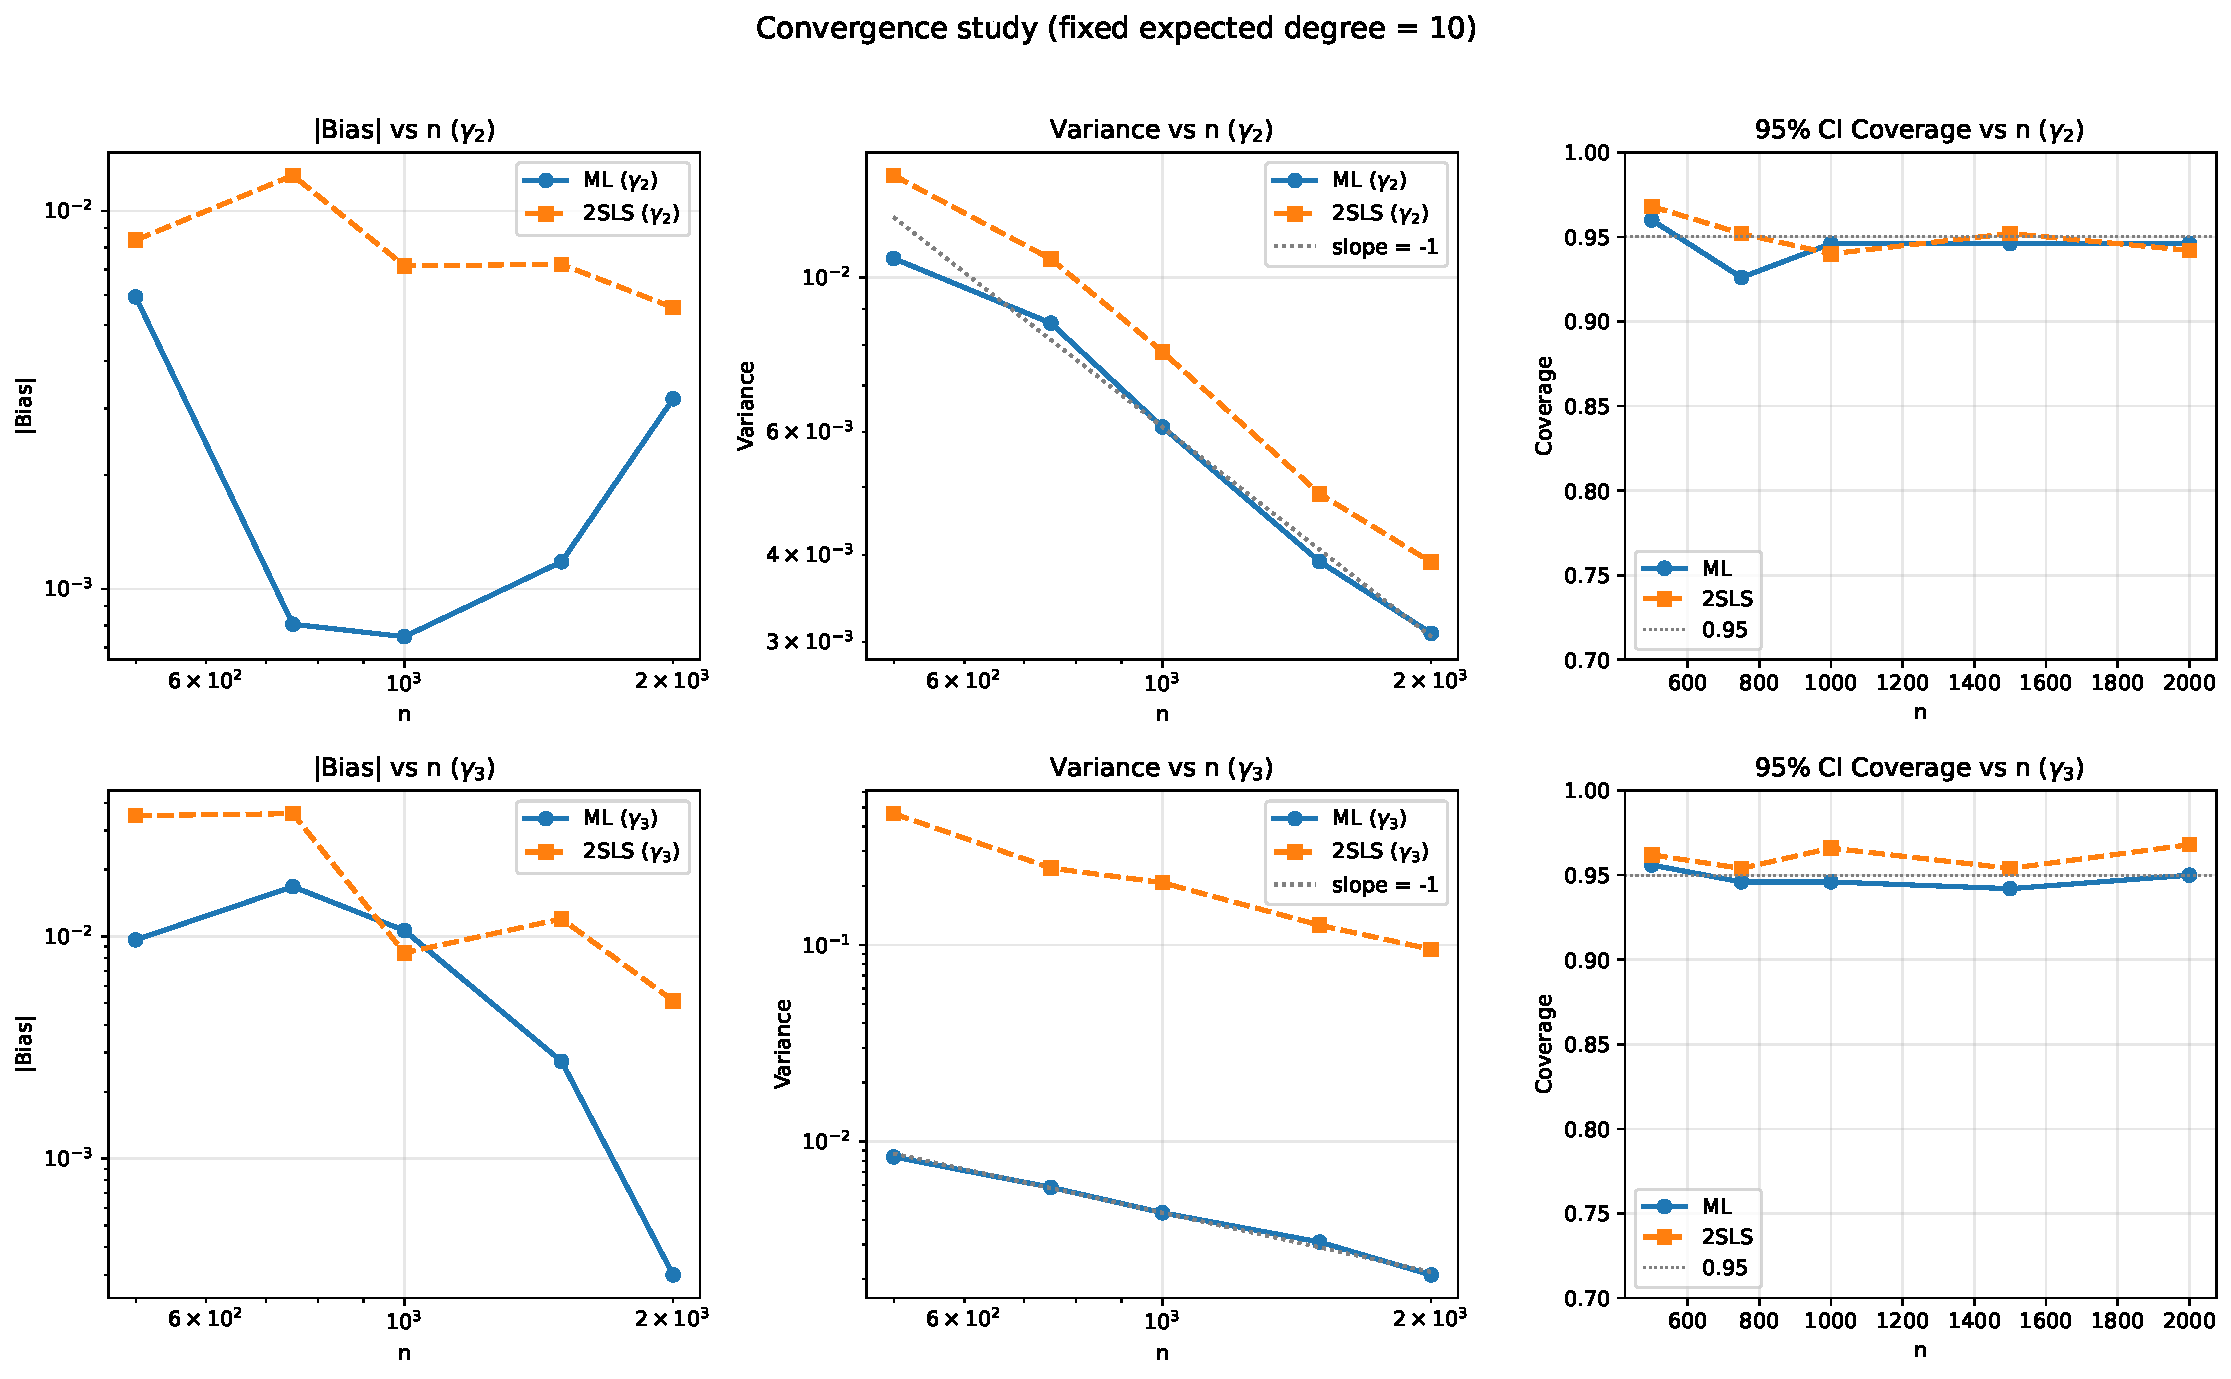
\includegraphics[width=\textwidth]{figures/mc_convergence.pdf}
    \caption[Convergence of ML and 2SLS estimators with sample size]{We display the convergence of ML and 2SLS estimators. The top row shows results for $\gamma_2$, the bottom row for $\gamma_3$. The plots show $|\text{Bias}|$ vs.\ $n$ on a log-log scale, variance vs.\ $n$ on a log-log scale, and $95\%$ CI coverage vs.\ $n$. We include a reference line at $0.95$, and grey dotted reference slopes ($-1$).}
    \label{fig:mc_convergence}
\end{figure}

Following the asymptotic theory review in Section~\ref{sec:est:regularity} for ML and Section~\ref{sec:est:wb_2sls} for 2SLS, we expect both estimators to become more precise as $n$ increases. The usual $\sqrt{n}$ asymptotics imply a reduction in variance of $O(n^{-1})$, which implies $\text{RMSE} = O(n^{-1/2})$. In a log-log plot such as Figure~\ref{fig:mc_convergence}, this corresponds to points following lines with a slope of $-1$ for variance as $n$ increases. The bias is expected to approach zero, while the coverage is expected to get closer to $0.95$ as $n$ increases.

We begin by looking at the results for the $\gamma_2$ parameter (Table~\ref{tab:mc_convergence_g2} and top row of Figure~\ref{fig:mc_convergence}). Here, both estimators show clear convergence as the RMSE values decrease monotonically, with variance following a slope of $-1$. The ML estimator's RMSE decreases from roughly $0.103$ when $n = 500$ to $0.056$ at $n = 2{,}000$. Similarly, the RMSE of the 2SLS estimator decreases from around $0.119$ to $0.063$. Both estimators have negligible biases at all sample sizes, with variation in both bias and coverage being attributable to Monte Carlo sampling errors. For example, for the coverage, $\sqrt{0.95 \times 0.05 / 500} \approx 0.010$ implies a two-standard-error band of approximately $0.93$ to $0.97$.

The results for $\gamma_3$ are similar (Table~\ref{tab:mc_convergence_g3} and bottom row of Figure~\ref{fig:mc_convergence}), showing clear convergence. For the ML estimator, RMSE decreases from $0.092$ to $0.046$, while for 2SLS it decreases from $0.683$ to $0.308$, both with variances following a slope of $-1$. While both estimators converge appropriately, the RMSE of the 2SLS estimator is much larger than the ML RMSE, in line with the results of weak instruments from the earlier density study (Section~\ref{sec:mc:density}). Bias remains negligible and coverage stays near the nominal level at all sample sizes, with variability within the Monte Carlo sampling error.

Hence, the simulations of this section show that both estimators become more precise as $n$ increases, with variances approximately following the standard $\sqrt{n}$-convergence rate when network degree is fixed.

%% Section 6.8: Summary of Findings
\section{Summary of Findings}
\label{sec:mc:summary}
The results of the Monte Carlo simulations provide us with the empirical validation needed for the estimators developed in Chapter~\ref{chap:estimation}. The results demonstrate that the estimators work correctly under the model assumptions.

We summarise the findings of this chapter in a condensed list and discuss the practical implications for model application.

\begin{enumerate}
    \item \textbf{Hessian verification}: Analytical derivations of Hessians in Sections~\ref{sec:est:screen_hessian} and~\ref{sec:est:wb_hessian} match numerical finite-difference approximations, validating the standard errors.

    \item \textbf{Consistency}: At $n = 500$, both the ML and 2SLS estimators recover true parameters with negligible bias.

    \item \textbf{Coverage}: At $n = 500$, both ML and 2SLS estimators achieve approximate $95\%$ confidence interval coverage. For ML, coverage falls between $0.944$ and $0.963$, while for 2SLS it falls between $0.964$ and $0.968$. The slight over-coverage of the 2SLS estimator is attributable to conservative standard errors as a consequence of moderate instrument strength.

    \item \textbf{Asymptotic normality}: Our results verify that for the ML estimators, standardised $z$-scores are close to $\N(0, 1)$ when $n = 500$, confirming that the asymptotic approximation from \textcite[Thm.~3.2, p.~1906]{Lee2004} holds.

    \item \textbf{Efficiency}: We show that the ML estimator is more efficient than 2SLS\@. Relative efficiency ranges from $1.21$ ($\gamma_2$) to $5.02$ ($\gamma_3$) in the $n = 500$ case. The higher relative efficiency of $\gamma_3$ can be explained by moderate instrument strength.

    \item \textbf{OLS bias}: Fitting an OLS estimator that ignores the endogeneity present in our model yields an estimate with substantial bias in $\hat\gamma_3$. Our estimators that take endogeneity into account do not suffer from the same problem.

    \item \textbf{Wald test calibration}: For both the ML and 2SLS covariance estimators, the Wald tests give empirical sizes within Monte Carlo error of the nominal $0.05$ level (ranging from $0.038$ to $0.050$). This provides evidence that the asymptotic approximations underlying Wald inference hold at $n = 500$.

    \item \textbf{Network density}: When network density increases, the mean first-stage $F$-statistic decreases sharply. Instruments weaken, and 2SLS estimator performance drops. The ML estimator is more robust to density changes, with low bias across all tested densities. In our base case (expected degree $\approx 5$), the $F$-statistic of $14.78$ exceeds the threshold of $10$, and both estimators perform well.

    \item \textbf{Convergence}: Holding the expected degree fixed at $10$ and increasing $n$ from $500$ to $2{,}000$ showed that both estimators converge in accordance with expected asymptotic theory. While RMSE decreases monotonically for $\gamma_3$ with both estimators, the 2SLS estimator exhibits roughly an order of magnitude larger RMSE than ML, consistent with weak instruments at this density.
\end{enumerate}

We provide a few practical recommendations based on these findings, which should be followed before applying the model to data. First, after implementing the analytical Hessian, verify correspondence with a numerical approach to check the implementation. Second, when fitting the model, apply both ML and 2SLS estimators as a robustness check. If parameter estimates disagree, this should be cause for investigation. In such cases, ML estimates should be verified by checking the plausibility of the normality assumption, while the 2SLS estimates should be verified by checking instrument strength. Lastly, before applying 2SLS, verify instrument strength by reporting the first-stage $F$-statistic (preferring ML estimates if $F < 10$ and normality is plausible), and check that the network is sparse enough. For networks with expected degree exceeding $\approx 10$, ML is preferred if normality is plausible.
